\chapter{Peg in hole}

In Chapter 3, we demonstrated that we could learn a search policy from demonstrations of human teachers for a task consisting of locating a wooden 
object on a table and successfully transfer it to a robot apprentice. The motivation behind our approach is that the intuition 
and knowledge exhibited by the human teachers, during the search, consists of a good balance between exploration and 
exploitation actions which then can be encapsulated in a generative Gaussian Mixture Model (GMM) and subsequently used as a control policy. The approach
is satisfactory if we are interested in extracting different behaviours present across the human teachers and reproduce 
them. If our objective is however to learn a policy with a unique behaviour which is optimal or at least close to optimality, then using  
the approach detailed in Chapter 3, as it is, will not necessarily result in a pro-efficient policy. The reason is that the GMM will model
both the good patterns exhibited by the human teachers and their mistakes. If the task is difficult and many possible solutions exist, such 
as it was the case in the blindfolded search task of the previous Chapter, many demonstrations will be necessary for search patters to be 
present and encoded in the GMM. If not it would have to be combined with another policy as we did in Chapter 3, with our Hybrid GMM-Greedy 
policy. In other words the task undertaken is implicitly encoded, as there is no cost function encoding the task which is optimised, in 
the GMM and as a result the taught behaviour has to be goal oriented and consistent, which is not always the case in a blindfolded search task. 

To overcome the above mentioned limitations, in this Chapter, we use a binary cost function as means of ranking demonstrations provided 
by the human teachers. We combine our PbD-POMDP approach with an Actor-Critic Reinforcement Learning (RL) framework which is close to 
Fitted-Value Iteration(FVI) and other experience replay methods, which we will refer to as RL-PbD-POMDP. Our objective 
is to not perform noisy explorative rollouts which is common to all RL approach and is their achille heel, but only rely on 
the data provided by the human teachers. We do not want to perform any autonomous exploration common in RL for three reasons. 
The first is that it is time consuming and is typically only applicable to RL problems in which an exhaustive exploration 
of the entire state or parameter space is feasible, such as in traditional RL problems like the inverted pendulum or mountain cart. 
The reason is that the universal exploration method used throughout RL is state independent (sometimes state dependent) white noise 
which will result in an entire exploration of the state space. This
is not practical or even feasible for the type of search problems were are considering. The second reason is that the 
exploration cannot be random because we are using a physical robotic system, and this would be dangerous. The third reason, 
and most important, is that we want to use the same amount of information for our RL-PbD-POMDP than we did for the PbD-POMDP approach. 
This is to strongly highlighting the fact that we can obtain an improved policy without the need of any additional information

%We chose a search and Peg-In-Hole (PiH) task
We analyse our RL-PbD-POMDP approach on a power-socket Peg-in-Hole (PiH) search task. In this task, human teachers must demonstrate 
to a robot apprentice how to search for and connect a plug to a power socket. The first component of the task, the search for the 
socket, is similar to the table-wooden block setup in the previous Chapter. What makes the difference is the connection of the  
plug to the power socket, the PiH component, which requires a higher level of precision to be able to achieve.

% Show figure of the task setup.
\begin{figure}[h]
  \centering
  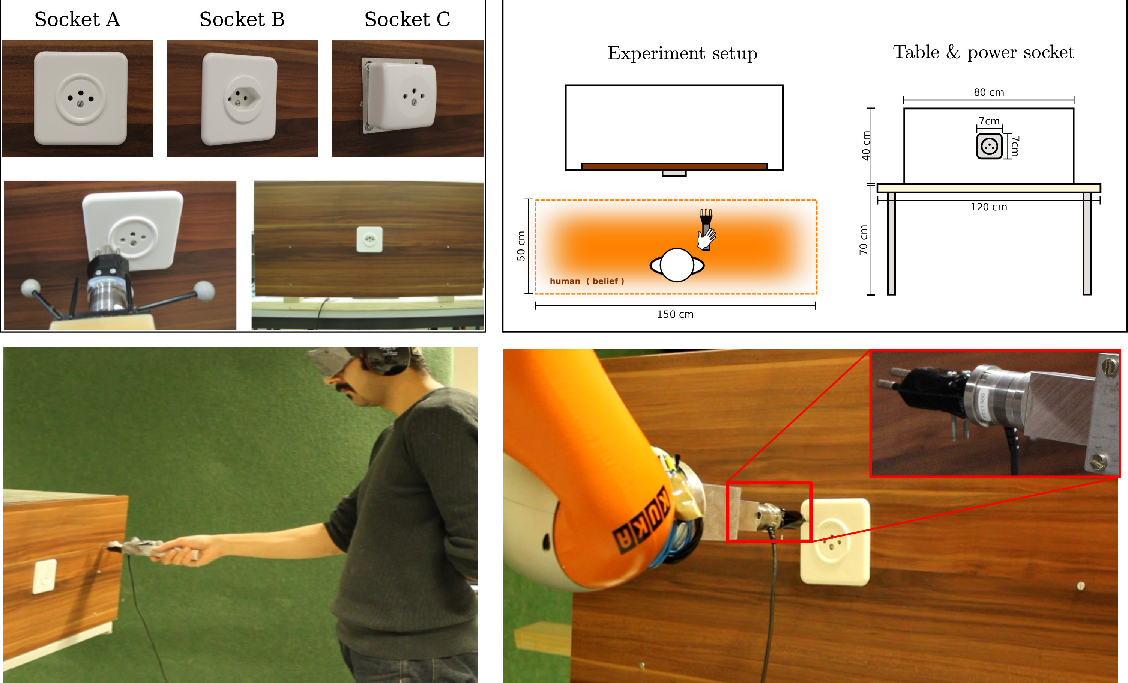
\includegraphics[width=0.95\textwidth]{./ch4-PiH/Figures/ex_setup_no_data.pdf}
     \caption{\textit{Top-right:} Experiment setup, blindfolded human subjects stand in the orange rectangle always 
   facing towards the table. Human subjects where informed of their starting location and where told that 
   they would always be facing the table. \textit{Top-left:} Three different powr sockets. The plug is connected
   to a cylinder such to make it easy to hold for the human subject. Between the cylinder and the peg is 
   an ATI 6-axis force torque sensor (Nano25 Series). \textit{Bottom-left} Human subject doing PiH search task. 
   The human subjects wore goggles to remove sight and wore ear defenders to greatly diminish 
   hearing.\textit{Bottom-right:} The KUKA LWR robot equipped with the same force torque sensor and plug that 
   the human subjects used during the demonstration phase.}
  \label{fig:experiment_setup}
\end{figure}

In Figure \ref{fig:experiment_setup} (\textit{Top-right}), we illustrate the setup of the search task. The digram shows
the distribution of the initial starting position (in orange) of the human teachers. As was the case in our previous search experiment
in Chapter 3, the teacher is disoriented before each trial but knowns that his initial heading will be the same, facing the wall. 
The human teachers are deprived of visual information (they are blindfolded) and their hearing sense is significantly 
reduced (they wear ear defenders).  We consider one type of plug, which is a Type J\footnote{http://www.iec.ch/worldplugs/typeJ.htm}, 
and three different power sockets. Power \textit{socket A}, has a ring around its holes, \textit{socket B} has a funnel, which we 
hypothesis should make it easier to connect, and \textit{socket C} has a flat elevated surface, see Figure \ref{fig:experiment_setup}
(\textit{Top-left}) for an illustration. The plug which the human teachers hold is attached to a cylindric handle with between the two 
an ATI 6 axis force torque sensor (Nano25 \footnote{http://www.ati-ia.com/products/ft/sensors.aspx}) is fixed and on top of the 
cylinder is a set of markers from which a motion capture system (OptiTrack\footnote{http://www.optitrack.com/}) provides
both position and orientation, see Figure \ref{fig:experiment_setup} (\textit{Top-left}). In the \textit{Bottom-left} quadrant we
can see an example of a human teacher trying to accomplish the search and connection and to the \textit{Bottom-right} the KUKA
LWR robot apprentice is reproducing a search policy learned from the teacher.


We found that by learning a value function over the belief space using approximate dynamic programming (part of FVI) and using 
this as a Critic to update the parameters of our GMM policy (Actor) we were able to achieve an important improvement over our 
previous PbD-POMDP approach. We  performed evaluations both in simulation and on the KUKA LWR robot in which we tested the ability of the policy to generalise
to sockets for which no training data was provided and different socket locations. In all our evaluations the RL-PbD-POMDP 
approach always proved to be better. More importantly we demonstrate that the RL-PbD-POMDP approach performs 
significantly better when we use the training data from the worst teacher, which is critical and mitigates the 
\textbf{original assumption}, that the teachers have to be consistently pro-efficient at the task.

\section{Outline}

\begin{itemize}
  \item \hyperref[ch4:background]{\ref{ch4:background}   Background}
  \item \hyperref[ch4:experiment]{\ref{ch4:experiment}   Experiment}
  \item \hyperref[ch4:formulation]{\ref{ch4:formulation} Formulation}
  \item \hyperref[ch4:results]{\ref{ch4:results}  	 Results}
\end{itemize}

\section{Background}\label{ch4:background}

\subsection{Peg-in-hole}

The Peg-in-Hole (PiH) task is one of the most widespread steps in industrial assembly and manipulations processes, with 
examples including the assembly of vehicular transmission components \cite{search_strategies_icra_2001} and 
valves \cite{online_gpr_icra_2014}. To be successful, the estimated
position of the robot's end-effector and workpiece must be precise. Typically the clearance between and peg and the workpiece's hole is very small, leaving 
little room for error. As a result, variations in the assembly's components in combination with position uncertainty 
can result in either jamming during the insertion process or the peg is unable to find the hole. This 
created a need for adaptive search and insertion policies for PiH, which has been driving research 
in this area. 

We identified, from the literature, the different components in PiH solutions. All approaches
use to some extend a vision system to estimate the position of the workpiece. Given an estimate of the workpiece's position, 
a common approach is to either follow a blind increasing spiral Cartesian trajectory or parametrised policies 
which guarantee that all positions on the workpiece have been visited. To 
increase the chance of a connection these approaches use a compliant controller, 
which usually includes a hybrid force/position controller.
The second predominant approach (which has been confined to academy) follows the data driven Programming by Demonstration (PbD) 
framework. Teleoperated or kinesthetic demonstrations of a human teacher are recorded and a policy is learned and fine tuned 
such to reproduce the same (F)orce/(T)orque profile as the ones demonstrated by the human teacher. The first approach 
does not consider reproducing the F/T profile but rather follows a position trajectory whilst being compliant.

In \cite{peg_personal_icra_2010} a PR2 executes a parameterised policy designed to connect a plug to a power outlet
in order for the PR2 to recharge itself. The plug was equipped with a checkerboard to facilitate pose estimation
of the peg with respect to power outlet who's position was extracted through a vision processing pipeline.
An initial connection was attempt by visual servoing which was successful 10\% of the time. When unsuccessful 
a spiralling outward motion with 2mm increments was carried out. They achieved an overall success rate of 95\%.
The hybrid control paradigm \cite{hybrid_1992} was used throughout the execution of the task.

% PbD: reproduce the F/T profile irrespective of the learned position trajectory DMP
In \cite{fast_peg_pbd_icmc_2014} the authors learned a PiH policy for the Cranfield benchmark object.
A vision system obtained the pose parameters of the object whilst a human teacher  
demonstrated trajectories, through teleoperation, in the frame of reference of the object. 
A time dependent policy represented with Dynamic Movement Primitives (DMP) \cite{Schaal04learningmovement} 
encodes the recorded Cartesian end-effector pose. A F/T profile is encoded separately by a regressor parameterised 
by radial basis functions. Successive refinements of the DMP policy are achieved through 
using force feedback to adapt the parameters of an admittance controller. This resulted in the policy having
a similar force profiles as the human teachers. Such an approach was first proposed by \cite{trans_workpiece_icra_2013}
and further applications based on this method have been done \cite{sol_pdg_pbd_2014} with the incorporation of  
a disturbance rejection policy.
Reinforcement learning has also been used in combination with DMP to learn PiH policies. In \cite{learn_force_c_icirs_2011}
an DMP policy is initialised with kinesthetic demonstrations of a door opening and pen pick up task. The recorded Cartesian trajectory
are encoded in parameterised DMP policy and augmented with a F/T regressor profile. A reward function is designed encoding desirable properties 
of the F/T profile such as smoothness and continuity and after a 110 trials a policy was found to be successful 100\% of the time.
In \cite{learn_admittance_icra_1994} a 18 dimensional (sensed position, previous position and force) input and 6 dimensional 
output (linear and angular velocity) neural network is learned by associative reinforcement learning. During the learning process the peg would be randomly 
positioned (both position and orientation) within the vicinity of the hole and after a 100 executions and 
updates, the policy was successful at the task and was able to generalise across different geometries and 
clearances. 

The policy of the above methods were learned from human demonstrations and encoded by a regressor function and
optimised to reproduce a desired F/T profile. The next approaches to the PiH problem 
are predominantly based on heuristic search mechanism and compliant controllers.

% Blind search stragegies
In \cite{search_strategies_icra_2001} different blind search policies for the insertion of a spline toothed hub 
into a forward clutch are analysed. The state space was discretised into points such that the distance between two 
neighbours was smaller than the clearance of the hole, which is known as a spray point coverage. Different search 
strategies which ensure that all the points are visited were evaluated. It was found that paths following a 
concentric circles gradually spiralling inwards were the most effective in finding the hole. The concentric circle
search strategy has been applied in many PiH tasks. For instance in \cite{peg_imcssd_2015}, a PiH heuristic 
policy was developed to connect a 5-pin water proof industrial charger to an electric socket. The authors 
estimated the pose of the socket through a vision system and use a force controller in combination with a 
spiral search policy to achieve a connection and demonstrated their approach to be reliable. 

% Do it the same way that humans do it: Does not use FT sensor
In \cite{intuitive_peg_isr_2013} the authors make the remake that humans do not have the precision and sensing 
accuracy of robotic systems, but nevertheless we are more proficient than robots at PiH. The authors make 
the observation that when humans try to connect a square peg to a socket, they rub the peg against the socket's 
outlet without looking. It is thought that the inherent compliance in humans motor control  
is key to our success at PiH tasks \cite{compliant_manip_icra_2008}. 
The authors introduce an Intuitive Assembly Strategy (IAS), inspired by the above observation, which 
does not require the hole to be precisely localised. The IAS search strategy is based on compliant 
spiral motion and the execution of the search trajectory is done with a hybrid force/position controller.

The spiral strategy is widely used in industrial applications due to its simplicity, 
however it is a blind search method. Another approach to the assembly process 
consists of fin tuning parameters of predefined policies. In \cite{online_gpr_icra_2014}
the author develops an online Gaussian Process parameter policy search of an assembly task. The authors
demonstrate that by learning the dynamics of the task during execution the model it is much more rapid in fine tuning 
the parameters in contrast with offline methods such as Design of Experiment (DOE) or Genetic Algorithms.

\subsection{Actor-Critic \& Fitted Reinforcement Learning}

The policy we learn to accomplish the search and socket connection is based on an Actor-Critic architecture
\cite[Chap. 6.6]{Sutton00policygradient}.


% Start by taking about updating the parameters
% What assume that value function has a different functional form 

% Convergence only guartees -> Policy Gradient theorem.

The advantage of an Actor-critic (AC) over a policy gradient method is that the variance of the
expected gradient estimate is lower. This means that the policy will converge quicker and there is less risk of divergence.

Learning Q and deriving a policy from it requires an online optimisation at every time step to find the optimal action.

% The lower variance is traded for a bias at the start of the learning when the estimates are far from accurate.

Actor-only policy methods, also known as policy search, converges is guaranteed if the estimated
gradients are unbiased (General policy gradient theorem). 

% Small changes in the value function will result in small changes in the policy

% Critic is usally updated via temporal difference error

Policy gradient theorem: 

\cite{rl_ac_surv_2012}

\cite{Sutton00policygradient} % Policy Gradient theorm

\cite{Boyan95generalizationin} % Safely approximiting the value function

\cite[Chap 6.6]{sutton98a}

% Explain why Actor-Critic is better 

\cite{rl_ac_surv_2012}

% % Explain why Fitted / Batch reinforcement learning is better 

\cite{fqi_nips_peter_2009},\cite{batch_synth_traj_2013},\cite{fnac_ca_2008},\cite{Riedmiller2005}, \cite{EGW05}, \cite{rl_gmm_2010}
\cite{fvi_uav_2010}
\cite{mnih-dqn-2015}
\cite{neura_fqi_2005}
\cite{DRQ_AAAI_2015}

\cite{approx_rl_overview_2011} % Appoximiate RL overview


\section{Experiment}\label{ch4:experiment}

The sockets are positioned at the center of a fake wall clamped to a table, see Figure \ref{fig:experiment_setup} (\textit{Top})
for an illustration of the environment. Each subject is given the opportunity to familiarise himself with 
the environment. Before each trial the human subject is placed on a chair and disoriented by the experimenter. Once disoriented,
the subject is allowed to stand and is signalled by a light touch to the shoulder to start the search task.
Figure \ref{fig:experiment_setup} (\textit{Middle-left}) illustrates a human subject doing the task. The disorientation
step is to induce the effect of an uniform prior over the subjects believed location. We make the assumption that the humans 
believed location can be presented by a probability density function, which we assumed to be known initially and that 
all subsequent distributions can be obtained through the application of a Bayesian filter given that we have both 
access to the sensing and motion information prided by the force torque and motion capture sensors.

In Figure \ref{fig:experiment_setup} (\textit{Top-right}) we illustrate the experiment setup. The orange area represents 
the starting location of the subject and is assumed prior knowledge. The subjects are told and shown before hand the environment setup
and it is made explicitly clear to them that they will always be starting in the orange area and will always be facing towards 
the wall. The area in which the human subjects would be starting was clearing demarcated on the floor by an adhesive band.

A group of 10 human subjects participated in the peg-socket experiment. The subjects performed the search and PiH 
for sockets A and B. A subject of group A (starting with socket A), would start by performing 15 times the search and connection 
with socket A and after a short break would carry on to perform 15 trials with socket B. During the break
the experiment changed the sockets on the fake wall.

Before the actual recording of the task, the subjects had a training period to familiarise themselves 
with environment and become comfortable wearing the sensor deprivation apparatus. After each subject felt sufficiently
ready to carry out the task to the best of his ability, the experimenter proceeded to disoriented him through 
the usage of a chair as mentioned previously. The subjects were reminded that they were facing the direction of 
the fake wall and that the staring location will always is the orange rectangular area. In Figure \ref{fig:experiment_setup_data}
we can see the time taken by the subjects to accomplish the task. 

It took $9\pm10$s for both Groups A and B to find the socket, which we expected since there is 
no difference in the setup when not considering the sockets. However after the socket was found it took $8\pm7$s on average to connect
socket B and $12\pm10$s on average to connect socket A. As we can see this is not a straight forward task when considering
the sensory deprivation, see Figure \ref{fig:experiment_setup_data} (\textit{Right}) for a detailed statistics regarding
the time taken to connect the plug to the socket.

\begin{figure}
 \centering
   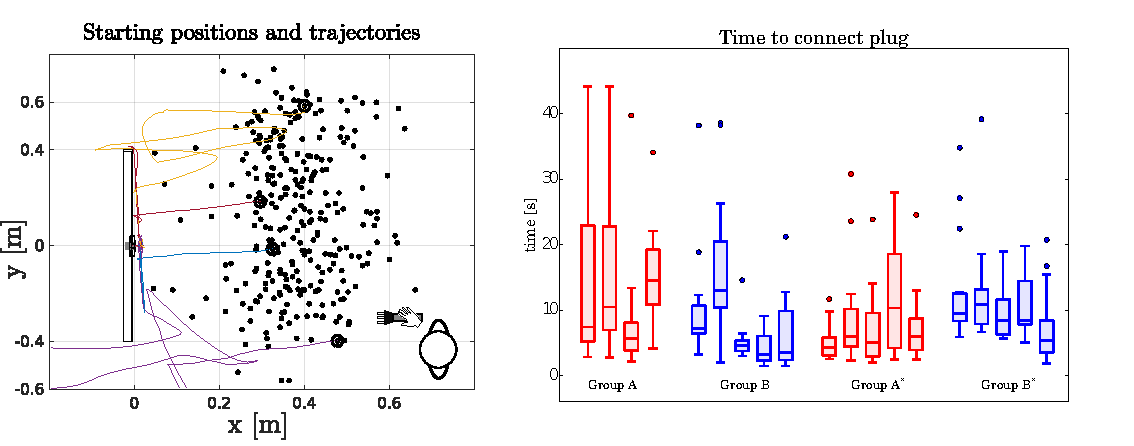
\includegraphics[width=\textwidth]{./ch4-PiH/Figures/ex_setup_data.pdf}
   \caption{\textit{Left}: black points represent the starting position of the end-effector
   for all the demonstrations, four trajectories are illustrated. \textit{Right:} 
   Time taken taken for the subjects to accomplish the PiH once the socket was localised. Group A and B are depicted in red 
   and blue. The asterisk indicates that the group is doing the task on the second socket, so Group A\textsuperscript{*} means
   that Group A is doing the task with socket B and Group B\textsuperscript{*} means that group B is doing the task with socket A.}
  \label{fig:experiment_setup_data}
\end{figure}

The location belief of the humans was represented by a probability density function. We made the assumption 
that after the disorientation step the human's believed location would be uniform and spread across the 
rectangular starting area which the subjects where informed of. It is not feasible to observe the 
mental state of the human, however there is sufficient evidence to support our assumption that his belief state
gets updated in a bayes like fashion [citation].

During each trial we recorded the position and orientation of the peg, provided by the motion capture 
system, and the sensed force and torque vectors, given by the ATI force torque sensor. 


\section{Formulation}\label{ch4:formulation}

\subsection{Belief probability density function}

In our setting the belief probability density function is a Point Mass Filter (PMF) \cite[p.87]{Bergman99recursivebayesian},
which is a  Bayes filter. It is parametrised by a set of grid cells  which contain valid probabilities.
Our choice of a PMF, as means to represent the believed location of the plug, is motivated by the fact that the 
sensing likelihoods are non-gaussian and lead to multi-modal distributions. A PMF is able to capture such non-gaussianity whilst
remaining fully deterministic (which is not the case for a particle filter).
The PMF gives probability density, $p(x_t|y_{0:t},\dot{x}_{0:t})$, which is recursively updated through the 
application of a \textbf{motion}, $p(x_t|x_{t-1},\dot{x}_t)$ and \textbf{measurement}, $p(y_t|x_t)$ model. 
The role of the motion model is to update the position of the probability density function and increase the uncertainty 
of the position. This step essentially consists of applying a convolution kernel to the PMF and we set the covariance 
of the kernel to proportional to the measured velocity.
The measurement model indicated areas of the state space in which a measurement $\tilde{y}_t$ could have originated from. Before explaining the measurement model we detail what  
measurement $\tilde{y}_t$ is. Both the human teachers and robot apprentice use the same sensor interface. This is a plug holder
equipped with a 6-axis force torque sensor which provides a sensed wrench, $\phi \in \mathbb{R}^6$, which we
call the \textbf{raw} measurement. We define the \textbf{actual} measurement to be a function of the sensed wrench, 
$\tilde{y}_t = h(\phi_t)$, which is a binary feature vector. The feature vector encodes whether a contact is present 
and the direction in which it occurs, which we discretized to the four cardinalities.
In Figure \ref{fig:PMF} (\textit{Right}) we illustrated the likelihood when an edge is sensed.

%The measurement model, $p(y_t|x_t)$, to be binary. If the peg enters in contact with the socket's edge 
%and the feature of $\tilde{y}_t$ corresponding to the left edge is active then the likelihood of regions close to the 
%left edge will be $1$, whilst others will be $0$.  %, another approach would to learn the model directly conditional distribution $p(\phi|x)$ from recorded data.

%\begin{figure}
% \centering
%   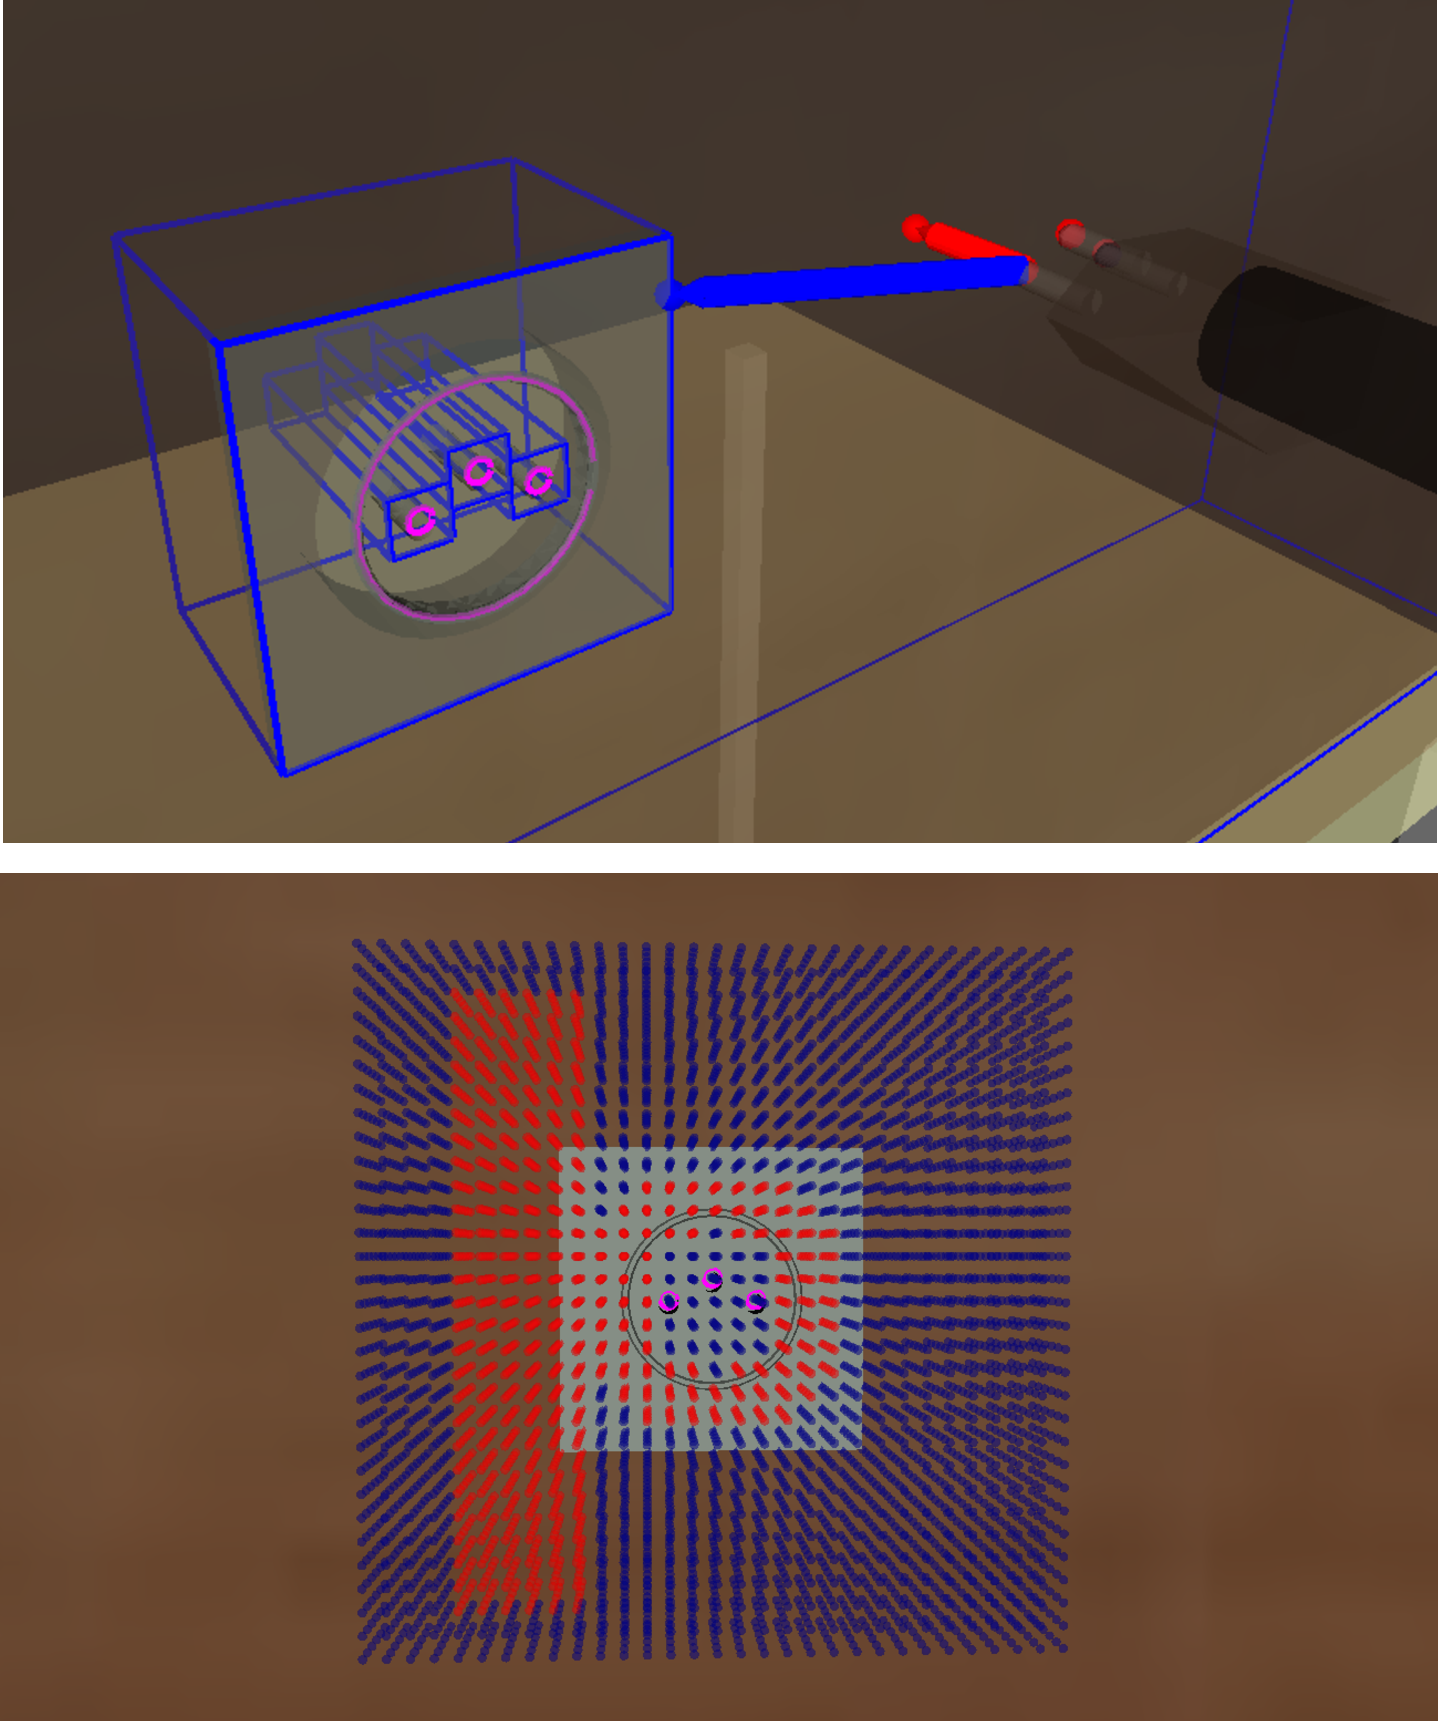
\includegraphics[width=0.45\textwidth]{Figures/images/measurement_model_2.pdf}
%   \caption{World model. \textit{Top}: The peg is presented by its three peg tips and the wall and sockets are fitted with bounding boxes 
%    The blue and pink lines represent edges and each surface is encoded by the equation of a plane. 
%    \textit{Bottom}: When the peg inters in contact with right edge of the socket the feature of the measurement vector $y_t$
%    corresponding to a contact coming from the right is $1$. As a result all the regions, $x_t$, close the left edge are one (red points)
%    whilst the others are zero (blue points) and areas around the socket's central ring are also set to one. 
%    }
%  \label{fig:world_model}
%\end{figure}

%We illustrate the likelihood for one type of contact, other contacts have there own likelihood function who's 
%activation depends on the current measurement. We do not consider the effect of noise since the measurements are binary. 
%This is one particular approach to define a measurement likelihood function amongst many others.
%  the feature of the measurement vector $y_t$ corresponding to a contact coming from the right is $1$.
%  the feature of the measurement vector $y_t$ corresponding to a contact coming from the right is $1$.
\begin{figure*}
 \centering
   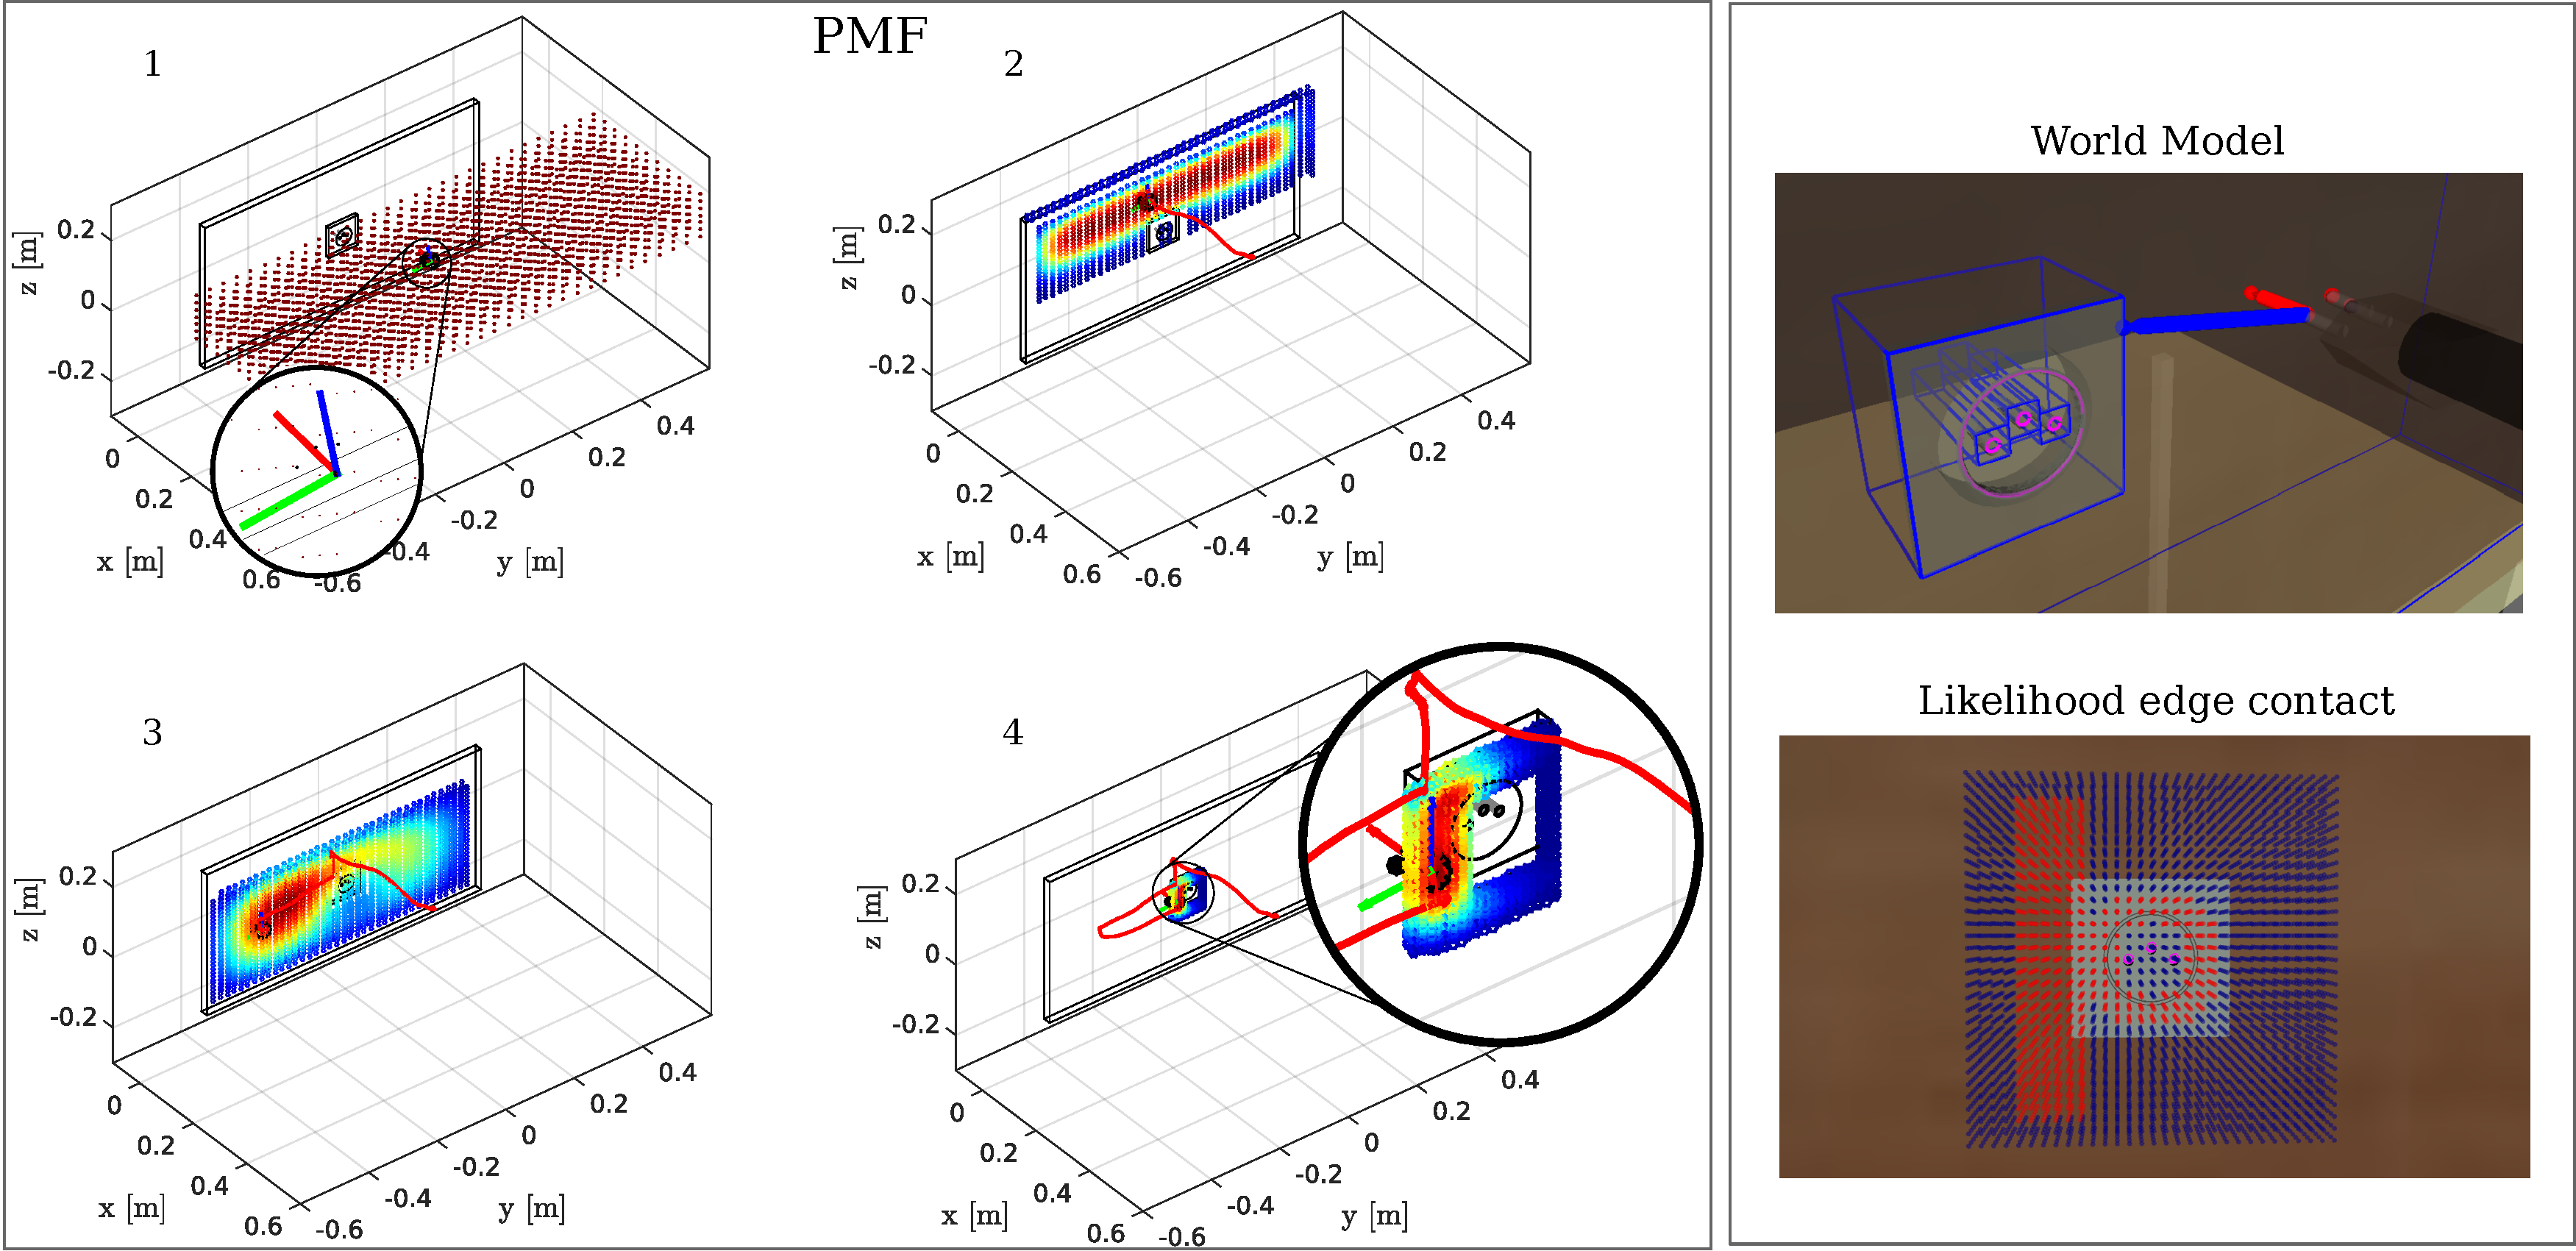
\includegraphics[width=\textwidth]{./ch4-PiH/Figures/PMF/pmf_likelihood.pdf}
   \caption{\textit{Left:} Point Mass Filter (PMF) update of a particular human demonstration. (1) Initial uniform distribution spread over the starting 
   region. Each grid cell represents a hypothetical position of the plug, the orientation is assumed to be known. (2) First contact, distribution is spread across the surface of the wall. The red trace 
   is the trajectory history. (3) motion noise increases the uncertainty. (4) The plug is in contact with a socket edge.
   \textit{Right}: \textbf{World model}: The plug is presented by its three plug tips and the wall and sockets are fitted with bounding boxes 
   \textbf{Likelihood}: When the plug inters in contact with right edge of the socket. As a result all the regions, $x_t$, close the left edge are one (red points)
    whilst the others are zero (blue points) and areas around the socket's central ring are also set to one. }
  \label{fig:PMF}
\end{figure*}

\subsection{Belief compression}

The probabilities density function $p(x_t|y_{0:t},\dot{x}_{0:t})$ is high dimensional and it is 
impractical to directly learn a statistical policy $\pi_{\theta} : p(x_t|y_{0:t},\dot{x}_{0:t}) \rightarrow \dot{x}_t$; 
some form of compression is necessary. A possibility would be E-PCA [cite] which finds a set of 
representative basis functions (which are probability distributions), although elegant this method 
requires a discretisation of the belief space which is computational expensive. Instead we chose to 
compress the pdf to belief space vector composed of the maximum a posteriori, $\hat{x}^{\mathrm{MAP}}_t = \argmax_{x_t} p(x_t|y_{0:t},\dot{x}_{0:t}) \in \mathbb{R}^3$, and the differentiation entropy, 
$U = H\{p(x_t|y_{0:t},\dot{x}_{0:t})\} \in \mathbb{R}$. All pdfs in our recorded data set $D$ are transformed to 
a belief space feature vector, $b_t = [\hat{x}^{\mathrm{MAP}}_t,U]^{\mathrm{T}}$. 

From the demonstrations we obtain a data set $D=\{\dot{x}^{[i]}_{1:T},\omega^{[i]}_{1:T},\phi^{[i]}_{1:T},b^{[i]}_{1:T}\}$, 
where the upper index $[i]$ references the ith trajectory and subscript $1:T$ denotes the time steps during the trajectory
from initialisation $t=1$ until the end $t=T$. The data consists of the peg's linear velocity, $\dot{x} \in \mathbb{R}^3$, 
angular velocity $\omega \in \mathbb{R}^3$, the sensed wrench $\phi \in \mathbb{R}^6$ (force-torque),
and the belief state, $b$, over the peg's location.

%probability distribution $p(x)$ over the believed location of the peg. Before going into details regarding the policy 
%to be learned, we introduce the formulation of probability density function, $p(x)$.
%The demonstrations gathered during the search for the socket entries, a priori to a connection being made, contain a wide spectrum of behaviour, 
%which at times appears to be stochastic and random. Learning directly a policy from this data, as it is often the case in LfD, 
%without a method for taking into account bad and good demonstrations will lead to a policy which will merely reproduce 
%the demonstrated behaviour including all its drawbacks. Our goal is to learn a policy which is optimal 
%in partially observable setting.


\section{Learning Actor and Critic}\label{sec:learning-value-actor}

In our approach we learn two data driven policies. The first maps from belief space 
to linear velocity $\pi_{\Para_1} : b_t \mapsto \dot{x}_t$ and the second from 
angular sensed wrench to angular velocity, $ \pi_{\Para_2} : \phi_t \mapsto \omega_t$.
We chose to learn the belief policy $\pi_{\Para_1}$ in a Actor-Critic RL framework 
and the wrench policy $\pi_{\Para_2}$ directly from the demonstrated data as was done 
in [cite], which proved to be efficient in overcoming jamming during the PiH. 
A POMDP solver's objective is to find a policy (Actor), $\pi_{\Para_1}: b \mapsto u$, which maximises 
the value function (Critic) $V^{\pi_{\Para_1}} : b \mapsto \mathbb{R}$ for an initial belief, $b_{0}$. The value function
is the expected reward over an infinite time horizon.
\begin{equation}\label{eq:value_function}
  V^{\pi_{\Para_1}}(b_t) = \mathbb{E}\Bigg\{ \sum_{t=0}^{\infty} \gamma^{t} r_{t+1} | b_0=b,\pi_{\Para_1}\Bigg\}
\end{equation}
In an actor-critic setting, the temporal difference error, $\delta_t \in \mathbb{R}$, of the value function (the critic) is used both 
as a learning signal to update itself and the actor (the policy) simultaneously. In our setting we will 
learn two separate policies, on for the linear velocity and the other for the angular velocity. 
The reason for this is that during most of the search, until it is time to connect the peg to the socket,
the orientation remains the same. When the peg has to be connected, due to jamming effects, it is necessary 
to control for the orientation. 

\subsection{Actor}
%Two control policies are learned; The first $\pi_{\Para_1}: b \mapsto \U$, maps belief state $b$ to linear velocity, 
%$\U$ and the second, $\pi_{\Para_2}: \phi \mapsto \omega$ , sensed wrench, $\phi$, to angular velocity, $\omega$.
%These actors/policies are parametrised by a Gaussian Mixture Model (GMM), Equation \ref{eq:GMM}.
Both actors/policies are parametrised by a Gaussian Mixture Model (GMM), Equation \ref{eq:GMM}.

\begin{equation}
 \pi_{\Para}(\U,\B) = \sum\limits_{k=1}^{K} \piK	    \cdot  g(\U,\B;\MuK,\SigK) \label{eq:GMM}
\end{equation}
The parameters $\Para = \{w^{[k]},\MuK,\SigK\}_{1,\dots,K}$, are the weights, means and covariances 
of the individual Gaussian functions, $g(.)$,
\begin{center}
$\MuK =  \begin{bmatrix} \MuK_{\U} \\ \MuK_{\B} \end{bmatrix}$, 
$\SigK =  \begin{bmatrix} 
	  \SigK_{\U\U} & \SigK_{\U\B} \\
	  \SigK_{\B\U} & \SigK_{\B\B}
	  \end{bmatrix}$
\end{center}
where $\sum_{k} w^{[k]} = 1$, $\MuK_{\U} \in \mathbb{R}^{3}$ and  $\MuK_{\B} \in \mathbb{R}^{4}$.
There are three steps in learning and then using for control a GMM model.  To learn a policy 
a generative model is learned through Expectation-Maximisation (EM) which maximised the likelihood
of the data. We learn a generative model of the angular velocity and wrench $\pi_{\Para_2}(\omega,\theta)$
and over the linear velocity and belief state $\pi_{\Para_1}(\dot{x},b)$. In both cases to determine the number 
of Gaussian functions we use the Bayesian Information Criterion. We will show how the parameters of $\pi_{\Para_1}$
can be adapted by the value function of the Critic in the next section.

%First a generative model, $p_{\Para}(\dot{x},b)$, is learned through maximising the likelihood of 
%the dataset by Expectation-Maximisation (EM). 
%Second the conditional is taken $p_{\Para}(\dot{x}|b)$
%giving a distribution over the applicable actions $\dot{x}$, Equation \ref{eq:GMC}

%\begin{equation} 
%  \pi_{\Para}(\U|\B) = \sum\limits_{k=1}^{K} \piK(\B) \cdot  g(\B;\MuK_{\U|\B},\SigK_{\U|\B}) \label{eq:GMC}
%\end{equation}
%\begin{align}
% w^{[k]}(\B)  &= \frac{\piK \cdot g(\B;\MuK_{\B},\SigK_{\B\B})}{\sum_{j=1}^{K} w^{[j]} \cdot g(\B;\Mu{j}_{\B},\Sig{j}_{\B\B}) } \\
% \MuK_{\U|\B}   &= \MuK_{\U} + \SigK_{\U\B} \invSigK_{\B\B}(\B - \MuK_{\B})\\
%  \SigK_{\U|\B} &= \SigK_{\U\U} - \SigK_{\U\B}\invSigK_{\B\B}\SigK_{\B\U}
%\end{align}
%Thirdly a concrete action, to be applied, is derived from the conditional distribution. One approach is
%to take the expectation of the conditional, $\hat{\U} = \mathbb{E}_{p_{\Para}(\U|\B)}\{\U\}$ whilst 
%another is to draw a sample $\U \sim p_{\Para}(\U|\B)$. 

\subsection{Critic}

% Q-learning and TD(0) are based on the dynamic porgramming algorithm known as value iteration.
% 
%\cite{NIPS2008_3501} (Fitted Q-iteration by Advantage Weighted Regression)
%
%We use a combination of function approximation and dynamic programming to learn a value function 
%of the belief state with respect to the given task.

%\cite{Szepesvari:2010}

The goal of the critic (the value function, Eq. \ref{eq:value_function}) is to evaluate 
the performance of the current policy. It is the expected future reward given the current 
belief state and policy.
In our setting we consider the case that a negative reward of $r=-1$ is received at each time step
until the goal (peg-socket connection) is achieved in which case a reward of zero is given, $r_{T}=0$.
Given the continuous nature and dimensionality of the belief space we use locally weighted regression \cite{Atkeson97locallyweighted}
(LWR) as a function approximator of the value function, $V^{\pi}(b)$. LWR is a memory-based non-parametric function 
approximator. It keeps as parameters a set of input-target pairs $\{(\B,r)\}$. When a value is 
queried, $\B$, a set of $p$ neighbouring points are chosen from the input space and are 
weighted according to a distance metric. The predicted output is then the result of a weighted 
least square of the $p$ points. Equation \ref{eq:W} is the distance function used where 
$D$ is diagonal matrix.

\begin{equation}\label{eq:W}
 W_{i,i}  = \exp\left(-\frac{1}{2}(\B - \B_i)^{\mathrm{T}}\, D^{-1} \, (\B - \B_i) \right)
\end{equation}
A new value is queried according to Equation \ref{eq:lwr_predict},
\begin{equation}\label{eq:lwr_predict}
  V^{\pi}(b) = \B \,(B^{\mathrm{T}} W B)^{-1} B^{\mathrm{T}} W \mathbf{r}
\end{equation}
where $B = (\B_1,\dots,\B_p)^{\mathrm{T}} \in \mathbb{R}^{(D\, \times\, p)}$, $W \in \mathbb{R}^{(p\, \times\, p)}$ is
a diagonal matrix, $\mathbf{r} = (r_1,\cdots,r_p)^{\mathrm{T}} \in \mathbb{R}^{(p\, \times\, 1)}$

%We chose this method because it is a safe regressor to use when estimating a value 
%function \cite{Boyan95generalizationin} and is very flexible since it is non-parameteric.

\subsubsection{Fitted Policy Evaluation}

To learn the value function we apply batch reinforcement learning\cite{EGW05}, also know as experience replay.
It is an offline method which applies multiple sweeps of the Bellman backup operator 
over a data set of tuples $\{(\Bi_t,\Ui_t,r^{[i]}_{t},\Bi_{t+1})\}_{i=1,\cdots,M}$ until the Bellman residual,
$||V^{\pi}_{k+1}(\B) - V^{\pi}_{k}(\B)||$, converges. 

\begin{algorithm} 
\caption{Fitted Policy Evaluation}
\label{alg:fpe}
\begin{algorithmic}[1]
    \Inputs{$K$, $\epsilon$, $\{(\B^{[i]}_t,r^{[i]},\B^{[i]}_{t+1})\}_{i=1,\cdots,M}$}
    \State{Initialise $\hat{V}^{\pi}_{0} = 0$}
    \For {$k=0$ in $K$}
        \State $\hat{V}^{\pi}_{k+1}(\B_t)$ = Regress($\B$, $r_t + \gamma \hat{V}^{\pi}_k(\B_{t+1})$)
	\If{$||\hat{V}^{\pi}_{k+1}(\B) - \hat{V}^{\pi}_{k}(\B)|| < \epsilon$ } 
	  \State \textbf{return} $\hat{V}^{\pi}_{k+1}(\B)$
	 \EndIf
    \EndFor
\end{algorithmic}
\end{algorithm}

A wide spectrum of research has made use of batch RL methods to learn a policies. 
Most of them have focused on learning the Q-value function (Fitted Q-Iteration) 
\cite{NIPS2008_3501,EGW05,Riedmiller05neuralfitted} directly. Although learning the 
Q-value function directly solves the control problem it often requires discretisation 
of the action space or assumes quantifiable actions. The reason is that doing 
Q-Bellman backups, $\hat{Q}(\B_t,\U_t) \leftarrow \gamma \max_{\U_{t+1}} \hat{Q}(\U_{t+1},\B_{t+1})$, 
requires an optimisation over the actions space, $\U_{t+1}$, to find the best applicable action. 
Given the dimensionality and continuity of our problem we opted for an on-policy evaluation method, 
which does not require an optimisation, but would require multiple 
\textit{policy evaluation} and \textit{policy improvements} iterations to achieve an optimal policy. 

%Which is not the case for Fitted Value Iteration (FVI) and Fitted Q-Iteration (FQI).
%After we applied the fitted policy evaluation to our dataset get the expected future 
%reward for each of the belief belief states, giving us a new dataset:
%$D = \big\{\U^{[i]}_{1:T},\omega^{[i]}_{1:T},\phi^{[i]}_{1:T},\B^{[i]}_{1:T},v^{[i]}_{1:T}\big\}^{i=1\dots N}$, where $v^{[i]}_t = \hat{V}^{\pi}(\Bi_t)$.

\begin{figure}
 \centering
 \setlength\fboxsep{0pt}
  \setlength\fboxrule{0.25pt}
  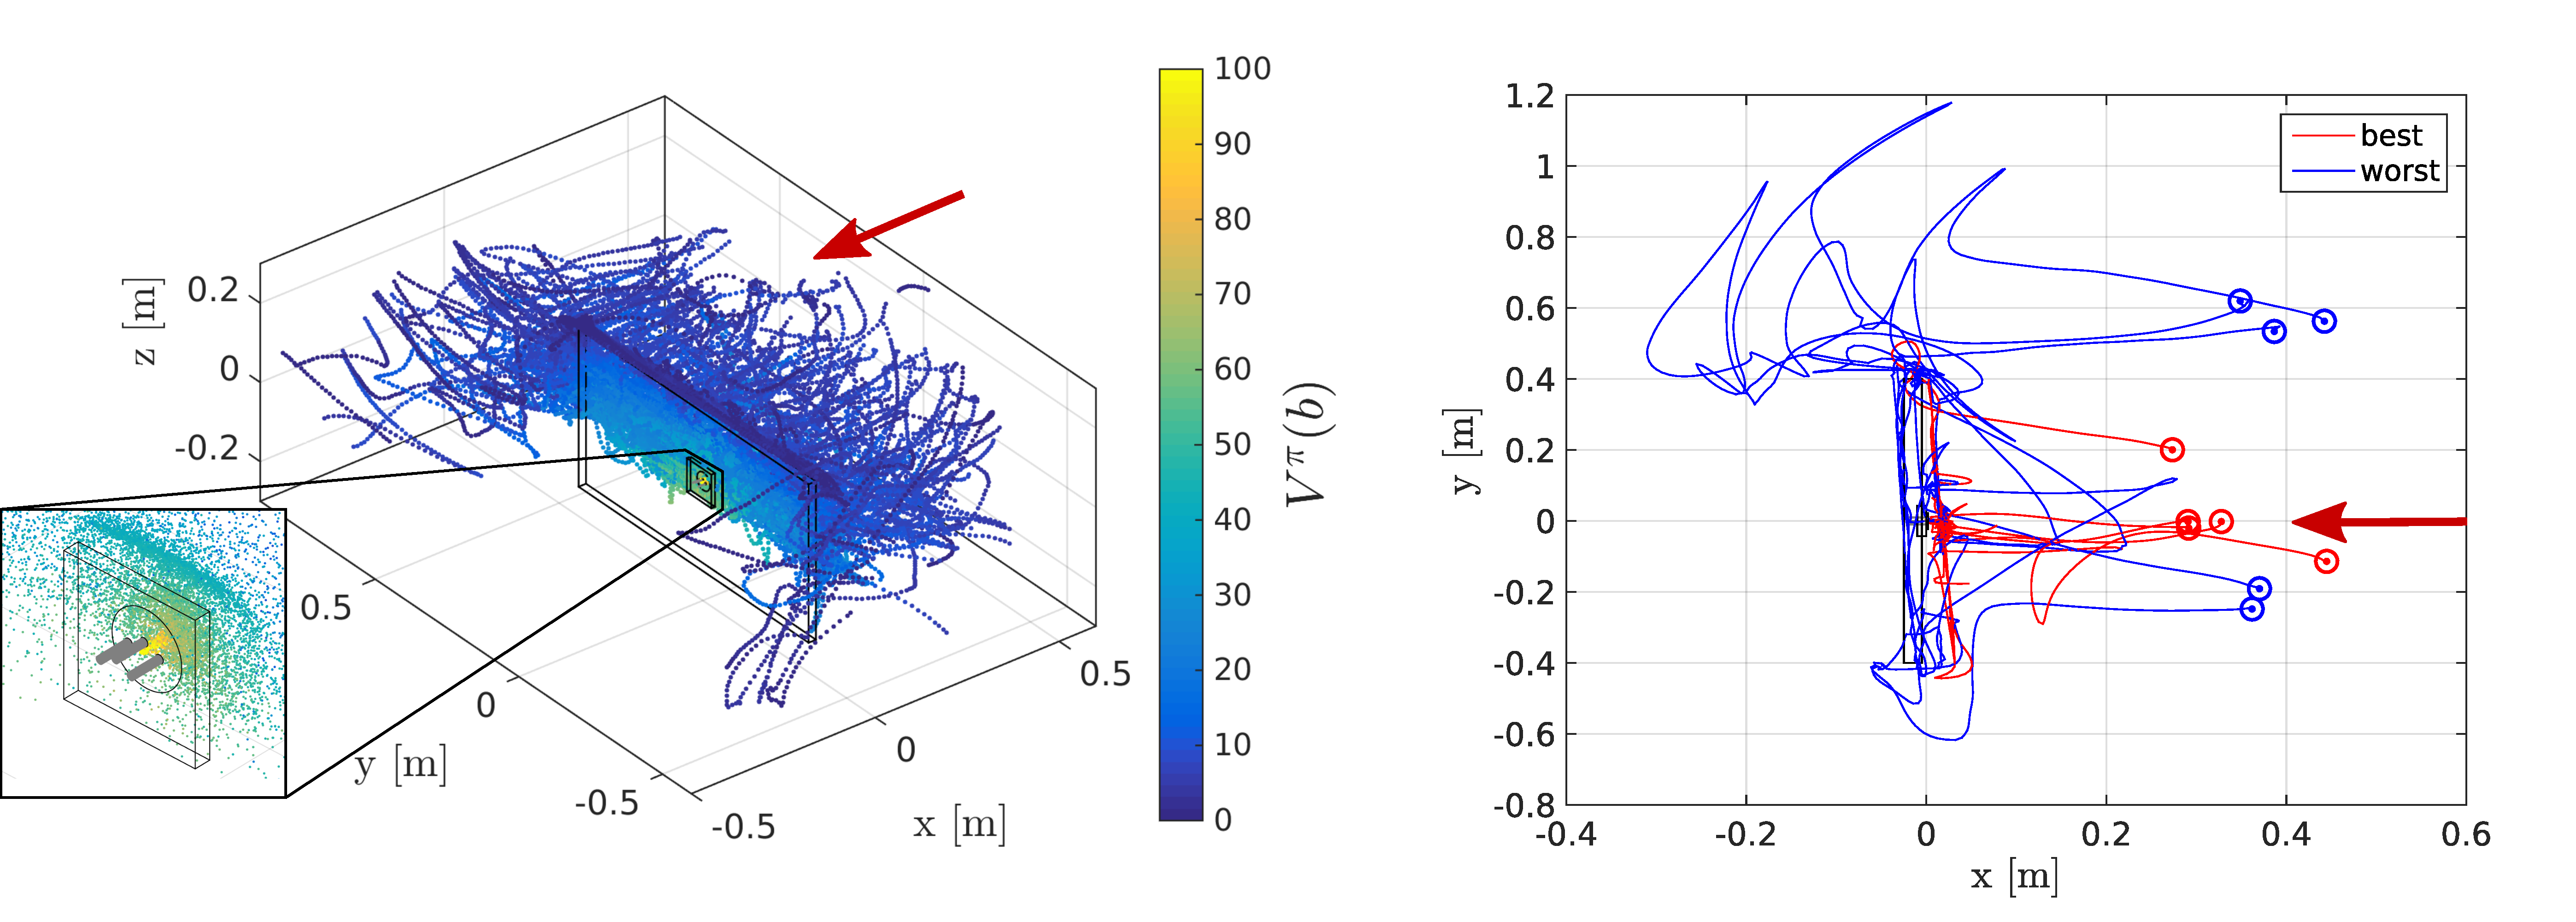
\includegraphics[width=0.8\textwidth]{./ch4-PiH/Figures/Figure1.pdf}
 \caption{\textit{Left:} LWR approximate value function $\hat{V}^{\pi}(\B)$. \textit{Right:} first five best and worst trajectories in terms accumulated value.}
  \label{fig:Figure1}
\end{figure}

In Figure \ref{fig:Figure1} (\textit{Left}) we plot belief space with the value function. We can see that as expected the 
value function is high close to the socket and low when further away. We show in Figure \ref{fig:Figure1}
(\textit{Right}) the best and worst trajectories in terms of accumulated value function are plotted. There is a
close relation to the time taken to successfully connect the peg to the socket. We can see that the five best trajectories
(red) tend to be aligned with the socket (star position in front of socket), whilst the five worst are towards the edges
of the wall. The critic having been learned can now be used to update the actor.

\subsection{Actor update}

The signal used to update the actor is the temporal difference error, 
$\delta^{\pi}_t = r_{t+1} + \gamma V^{\pi}(b_{t+1}) - V^{\pi}(b_t)$, given by the critic\cite[Chap. 6]{sutton1998reinforcement}. 
In our offline approach we first computed the value function of the belief state, $V^{\pi}(\B)$, 
until convergence and then use the estimated value function to update the actor. This offline batch 
method has the advantage that no divergence will occur during the learning.

We proceed to update the actor given the critic through a modification of the Maximisation step in  Expectation-Maximisation (EM) 
for Gaussian Mixture Models. We refer to this modification as Q-EM which is strongly related to a Monte-Carlo EM-based policy 
search approach \cite[p.50]{DeisenrothNP2013}. 

The reward of a demonstrated trajectory (one episode) is given by the discounted return, Equation $\ref{eq:disc_return}$.
\begin{equation}\label{eq:disc_return}
 R(\B^{[i]},\U^{[i]}) = \sum_{t=0}^{\mathrm{T^{[i]}}} \gamma^t \, r(\B^{[i]}_t,\U^{[i]}_t)
\end{equation}
All policy gradient approaches seek to find a set of parameters, $\Para$, of the actor
which will maximise the expected reward, equivalent to maximising Equation \ref{eq:expected_reward}.
\begin{align}\label{eq:expected_reward}
 J(\Para) &= \mathbb{E}_{\pi_{\Para}(\U,\B)}\{R(\B,\U)\} \nonumber \\
	  &= \sum\limits_{i=1}^{N}   \underbrace{\left( \prod_{t=0}^{T^{[i]}} \pi_{\Para}(\U^{[i]}_t,\B^{[i]}_t) \right)}_{\pi_{\Para}(\U^{[i]},\B^{[i]})} \, R(\B^{[i]},\U^{[i]}) 
\end{align}

To find the parameters which maximise the cost function, $\argmax_{\Para'} J(\Para')$, we take the derivative and 
set it to zero. This cannot be done directly and we have to resort to maximising the lower bound of the logarithm 
of the cost function. This results in Equation \ref{eq:grad_log_cost},

\begin{equation} \label{eq:grad_log_cost}
    \nabla_{\Para'}\log(J(\Para')) = \sum\limits_{i=1}^{N} \sum\limits_{t=0}^{T^{[i]}} \nabla_{\Para'}\log \pi_{\Para'}(\U^{[i]}_t,\B^{[i]}_t) \, Q^{\pi}(\U^{[i]}_t,\B^{[i]}_t)
\end{equation}

Setting the derivative of Equation \ref{eq:grad_log_cost} to zero and solving for the parameters
$\Para=\{w,\boldsymbol{\mu},\boldsymbol{\Sigma}\}$ leads to a Maximisation update step of EM
which is weighted by $Q^{\pi}$, see Appendix \ref{app:lb} for a more complete derivation.
We instead use the temporal difference error of the \textit{Critic} as a substitute 
to $Q^{\pi}$. If we assume that our estimated value function, $\hat{V}^{\pi_{\Para}}$, is close to the true value function 
$V^{\pi_{\Para}}$, the temporal difference error $\delta^{\pi}$ is an unbiased estimate of the advantage function, Equation \ref{eq:advantage_f} 
(see Appendix \ref{app:unbiased_delta}).
\begin{equation}\label{eq:advantage_f}
 A^{\pi}(b_t,u_t) = Q^{\pi}(b_t,u_t) - V^{\pi}(b_t) = \delta^{\pi}_t
\end{equation}
Using the advantage function as means of policy search is popular with examples such as
Natural Actor Critic (NAC) \cite{peter_nac_2008}.

Each data point has an associated weight, $\delta \in \mathbb{R}$, which when grater than zero, $\delta^{[m]} \geq 0$, means that the 
state action-pair $\X^{[m]}$ lead to an increase in the value function and if $\delta^{[m]} \leq 0$ lead to 
a loss. The likelihood is re-weight accordingly giving more importance to data points which lead to a gain. Since 
the Q-EM update steps cannot allow negative weights, we resale the temporal difference error to be between 0 and 1.

%We learn the peg-socket search policy using the Q-EM update rules for a GMM parametrisation with the 
%data set, $D_1 = \big\{\U^{[i]}_{1:T},\B^{[i]}_{1:T},\delta^{[i]}_{1:T}\}^{i=1\dots N}$ and learn a second policy for inserting the 
%final steps of connecting the peg to socket with data set $D_2 = \{\omega^{[i]}_{1:T},\phi^{[i]}_{1:T}\}^{i=1\dots N}$. 
%In Figure \ref{fig:data_flow} we illustrate the data flow and the policies which are learned. Note that we also learn a belief space 
%policy directly from the demonstrations, $\pi_{\Para_3}(\U,\B)$, which we will refer to as the GMM policy and we will use it to compare 
%with the policy corrected by the Critic, which we call the Q-EM policy.
%\begin{figure}[h]
%  \centering
%  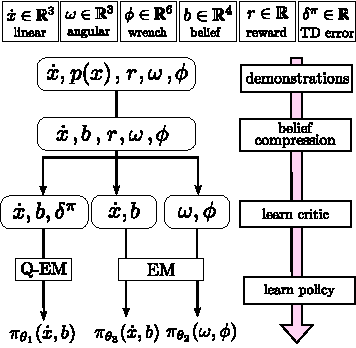
\includegraphics{Figures/data_flow_2.pdf}
%  \caption{Data flow and policies learned. The original data consists of five variables which are recorded during the demonstrations given 
%  by the human teachers. The probability density function of the believed location of the end effector is compressed to a belief state, which 
%  is the most likely state and entropy. The value function is learned via fitted policy iteration and each data point has a temporal difference 
%  error. An actor policy is learned via Q-EM, $\pi_{\Para_1}(\U,\B)$ , a regular policy is learned via the standard EM approach, $\pi_{\Para_3}(\U,\B)$
%  and a peg insertion policy is learned $\pi_{\Para_2}(\U,\B)$.}
%  \label{fig:data_flow}
%\end{figure}

\section{Control architecture}\label{seq:control_architecture}

We learned both a Gaussian Mixture Model of both the linear and angular 
velocity. For most of the search, until the peg's are within the socket's holes, only 
the linear control policy is active and the orientation is kept constant.

The direction to search is given by conditioning 
the belief dimension of the GMM, $\pi_{\Para}(\dot{x},b)$ resulting in a new 
probability distribution, Equation \ref{eq:gmm_conditional}.

\begin{equation}\label{eq:gmm_conditional}
 \pi_{\Para}(\dot{x}|b) = \sum_{k=1}^{K} w^{[k]}_{\xb} \cdot g(\dot{x};\MuK_{\xb},\SigK_{\xb})
\end{equation}

It is a distribution over the possible velocities, which are 
normalised. The subscript $\xb$ indicated the the parameters 
are the result of the conditional, the reader is referred to \cite{gesture_calinon_2010},\cite{gmr_2004} for 
a detailed derivation of the conditional of a GMM. In the autonomous
dynamical systems control the velocity to apply would be taken from 
the expectation of Equation \ref{eq:gmm_conditional}. The model 
which learn is multi-modal, different search velocities are possible 
in the same belief state, and taking the expectation, which is weighted 
linear combination of the modes would result in unobserved behaviour or 
none if the velocities cancel themselves out. In Figure \ref{fig:policy_vf}
we illustrate the multi-modal vector fields of the conditional, Equation \ref{eq:gmm_conditional}.
As a result we use a modified version of the expectation operator which favours the current
direction, Equation \ref{eq:alpha_eq} - \ref{eq:alpha_expectation}.

\begin{align}
 \alpha(\dot{x}) &= w^{[k]}_{\xb} \cdot \exp(-\cos^{-1}(<\dot{x},\MuK_{\xb}>)) \label{eq:alpha_eq}\\
 \dot{x} &= \mathbb{E}_{\alpha}\{\pi_{\Para}(\dot{x}|b)\} = \sum_{k=1}^K \alpha_k(\dot{x}) \cdot \MuK_{\xb} \label{eq:alpha_expectation}
\end{align}

When a velocity mode being applied is no longer present (because we have moved into a region of belief space where the current applied 
velocity has not been seen) another direction mode is sampled. An example occurs when the robot suddenly enters in contact with a feature
which greatly reduces the uncertainty and the current modes will dramatically change and hence a new search direction will then 
be computed. 

The above steps control the general behaviour of the search which is not sufficient for a successful implementation on a robotic system, such 
as the KUKA LWR.
This search task is haptic and as a result the end-effector of the robot will always be in contact with the environment. To make the robot
compliant with the environment we use an impedance controller in combination with a hybrid position-force controller. Our hybrid controller
targets a sensed force $F_x$, in the $x$-axis, of 3N. The other two velocity components of the direction vector are given by 
Equation \ref{eq:alpha_expectation}.This by itself was insufficient to reliably get over the edges of the socket; the robot 
would get stuck at edges unable able to overcome the friction as these right angle contacts. To overcome this we locally modulated 
the vector field of the GMM in $y$ and $z$-axis, Equation \ref{eq:modulation}.

\begin{equation}
  \dot{x} = R_y(c(F_z) \cdot \pi/2) \cdot R_z(c(F_y) \cdot \pi/2) \cdot \dot{x} \label{eq:modulation}
\end{equation}

$R_y$ and $R_z$ are rotation matrix around the $y$ and $z$-axis, $c(F) \in [-1,1]$ is a truncated scaling function of the sensed 
force.  When a force $F_z$ of 5N is sensed the rotation will be $R_y(\pi/2)$ applied to the original direction resulting in the robot
getting over the obstacle. The direction velocity is always normalised up to this point. The amplitude of the velocity is a proportional
controller based on the believed distance to the goal,
\begin{equation}
  \nu = \max(\min(\beta_1,K_p (x_g - \hat{x}),\beta_2)\label{eq:prop_speed}
\end{equation}
where the $\beta$'s are lower and upper amplitude limits, $x_g$ is the position of the
goal, and $K_p$ the proportional gain which was tuned through trials. In Figure \ref{fig:control_flow}
we illustrate the complete control flow.

\begin{figure}
  \centering
  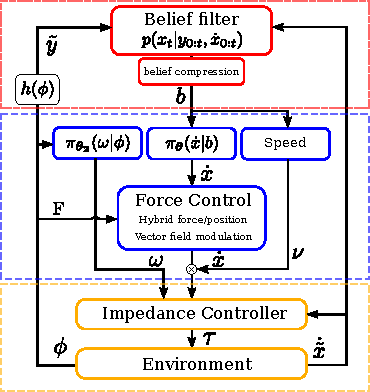
\includegraphics[width=\textwidth]{./ch4-PiH/Figures/control_flow_final.pdf}
  \caption{Control architecture. The PMF (belief) received a measured velocity, $\dot{\tilde{x}}$, and sensor feature $\tilde{y}$ and gets updated 
  via Bayes rule. The belief is compressed and used by both the GMM policy and the proportional speed controller, Equation \ref{eq:prop_speed}.}
  \label{fig:control_flow}
\end{figure}

\begin{figure}
   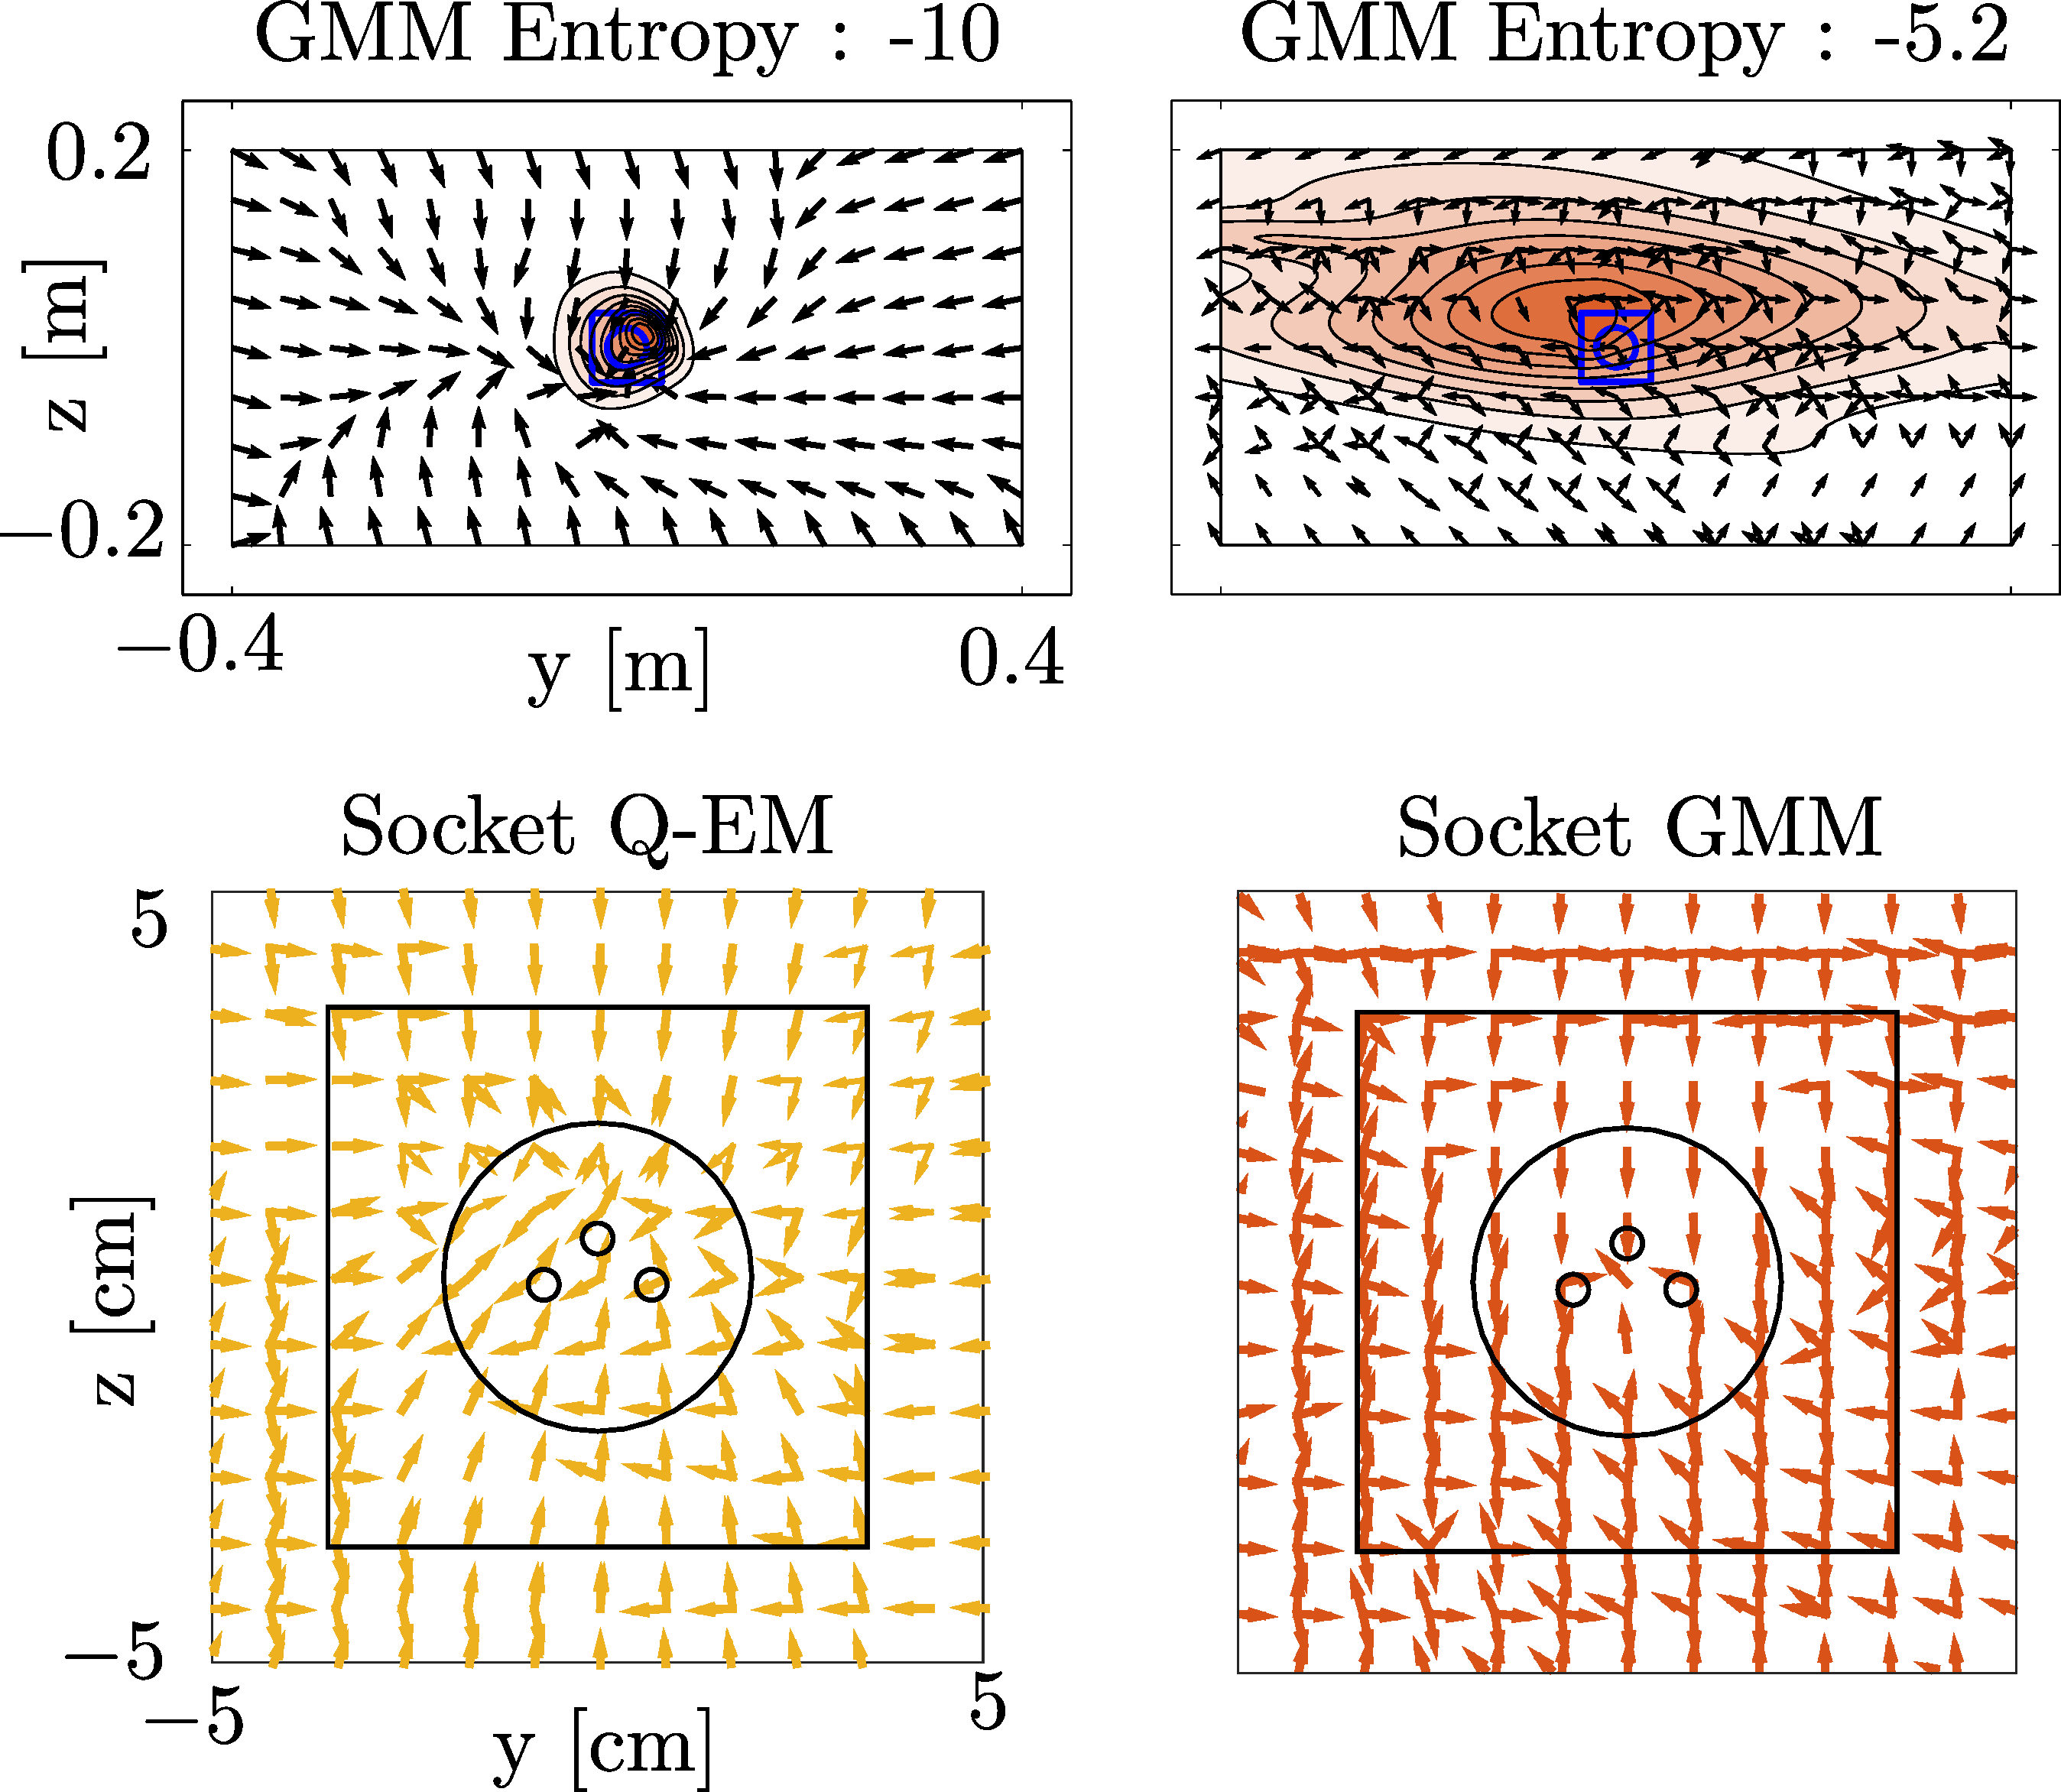
\includegraphics[width=\textwidth]{./ch4-PiH/Figures/Qualitative/policy_vf.pdf}
  \caption{Q-EM and GMM policy vector field. \textit{Top}: The GMM policy is conditioned on an entropy of $-10$ and $-5.2$. For the lowest entropy level,
  most of the probability mass is close to the socket area, since this level corresponds to very little uncertainty; we are already localised. We can see 
  that the policies vector converges to the socket area regardless of the location of the believed state. For an entropy of $-5.2$ we can see that 
  the likelihood of the policy is present across wall. The vector filed directs the end-effector to go towards the left or right edge of the wall. 
  \textit{Bottom}: The entropy is marginalised out, the yellow vector field is of the Q-EM and orange of the GMM. The Q-EM vector field tends 
  to be closer to a sink and there is less variation.}
  \label{fig:policy_vf}
\end{figure}

\FloatBarrier
\section{Results}\label{ch4:results}

We evaluate the following three properties of the policy learned in our Actor-Critic framework:
\begin{enumerate}
 \item \textbf{Distance taken to accomplish the goal} (connect peg to socket). We compare the Q-EM policy with 
 a GMM policy learned through standard EM and a myopic Greedy policy. This highlights the difference between complicated and simplistic  
  search algorithms and as a result gives an appreciation of the problem's difficulty.
 \item \textbf{Importance of data}, provided by human teachers. We evaluate whether it is possible to improve 
 the Greedy policy by using data collected from it. We use this data to learn a new GMM policy which we call 
 Q-Greedy. This is to test whether it is necessary to use a human teacher instead of using heuristics to 
 gather demonstrations.
 We evaluate whether it is possible to obtain a good policy from the worst two teachers. Not all teachers 
 are necessarily proficient at the task in question and we want to test whether our methodology can be applied in these
 cases. We evaluate if we  are able to obtain an improved policy from the worst two teachers.
 \item \textbf{Generalisation}. We learn a policy to insert a peg into socket A which was located at the center of the wooden 
 wall. We test the generalisation of the policy in finding a new socket location. We further test whether the policy can generalise to two new sockets 
 which were not used during the training phase.
\end{enumerate}

We evaluate the above properties under two separate conditions. In the \textbf{first condition} we consider the period between the start 
of the search until the socket is localised. In the \textbf{second condition} we consider the period from the point the socket is found until
a connection has been established. In the first condition the evaluation is done in simulation whilst 
in the second condition, when the socket is found, we perform the evaluation with a physical robot, the KUKA LWR4.

This choice is motivated by the fact that the task requires different levels of precision to accomplish it.
Finding the socket requires much less precision than establishing a connection. It is thus
more informative to consider the performance of these two parts separately.
Another aspect is that the search for the socket can be reliably evaluated in simulation since the physics of the interaction
are simple, whilst the connection phase is more complicated and using a simulation would be unrealistic.
For the evaluation of the connection of the peg to the socket we consider search initialisation already within 
the vicinity of the socket.

\subsection{Distance taken to reach socket's edge (Qualitative)}

We consider three search experiments which we refer to as \textbf{Experiment 1, 2} and \textbf{3},
in order to evaluate the performance, in terms of distance travelled to reach the socket, of three search policies: GMM, Q-EM and Greedy.
In these three experiments the task is considered accomplished when a search policy finds the socket's edge. 

In search \textbf{Experiment 1}, three starting locations are chosen: \textit{Center}, \textit{Left} and \textit{Right}, 
see Figure \ref{fig:box_exp_sim}, \textit{Experiment 1}, for an illustration of the initial condition. 
This setup tests if starting in front, to the left or right of the socket results in a difference between the search policies. 
A total of 25 searches are carried out for each of the search policies and the three starting initial conditions.

In \textbf{Experiment 2}, two \textit{Cases} are chosen in which the believed state (most likely state of the PMF) and the true position
of the end-effector are far apart. The location of the beliefs are chosen to be symmetric, see the Figure \ref{fig:box_exp_sim}, 
\textit{Experiment 2}. A total of 25 searches are carried for each of the two conditions.

In \textbf{Experiment 3}, Figure \ref{fig:box_exp_sim}, \textit{Experiment 3}, the initial true starting positions 
of the end-effector are taken from a regular grid covering the whole start region, also used as the initial distribution for 
the human demonstrations. A total of a 150 searches are carried out for each of the three policies. 
This experiment allows a comparison of the search policies with the human teachers.

\begin{figure}
    \centering
    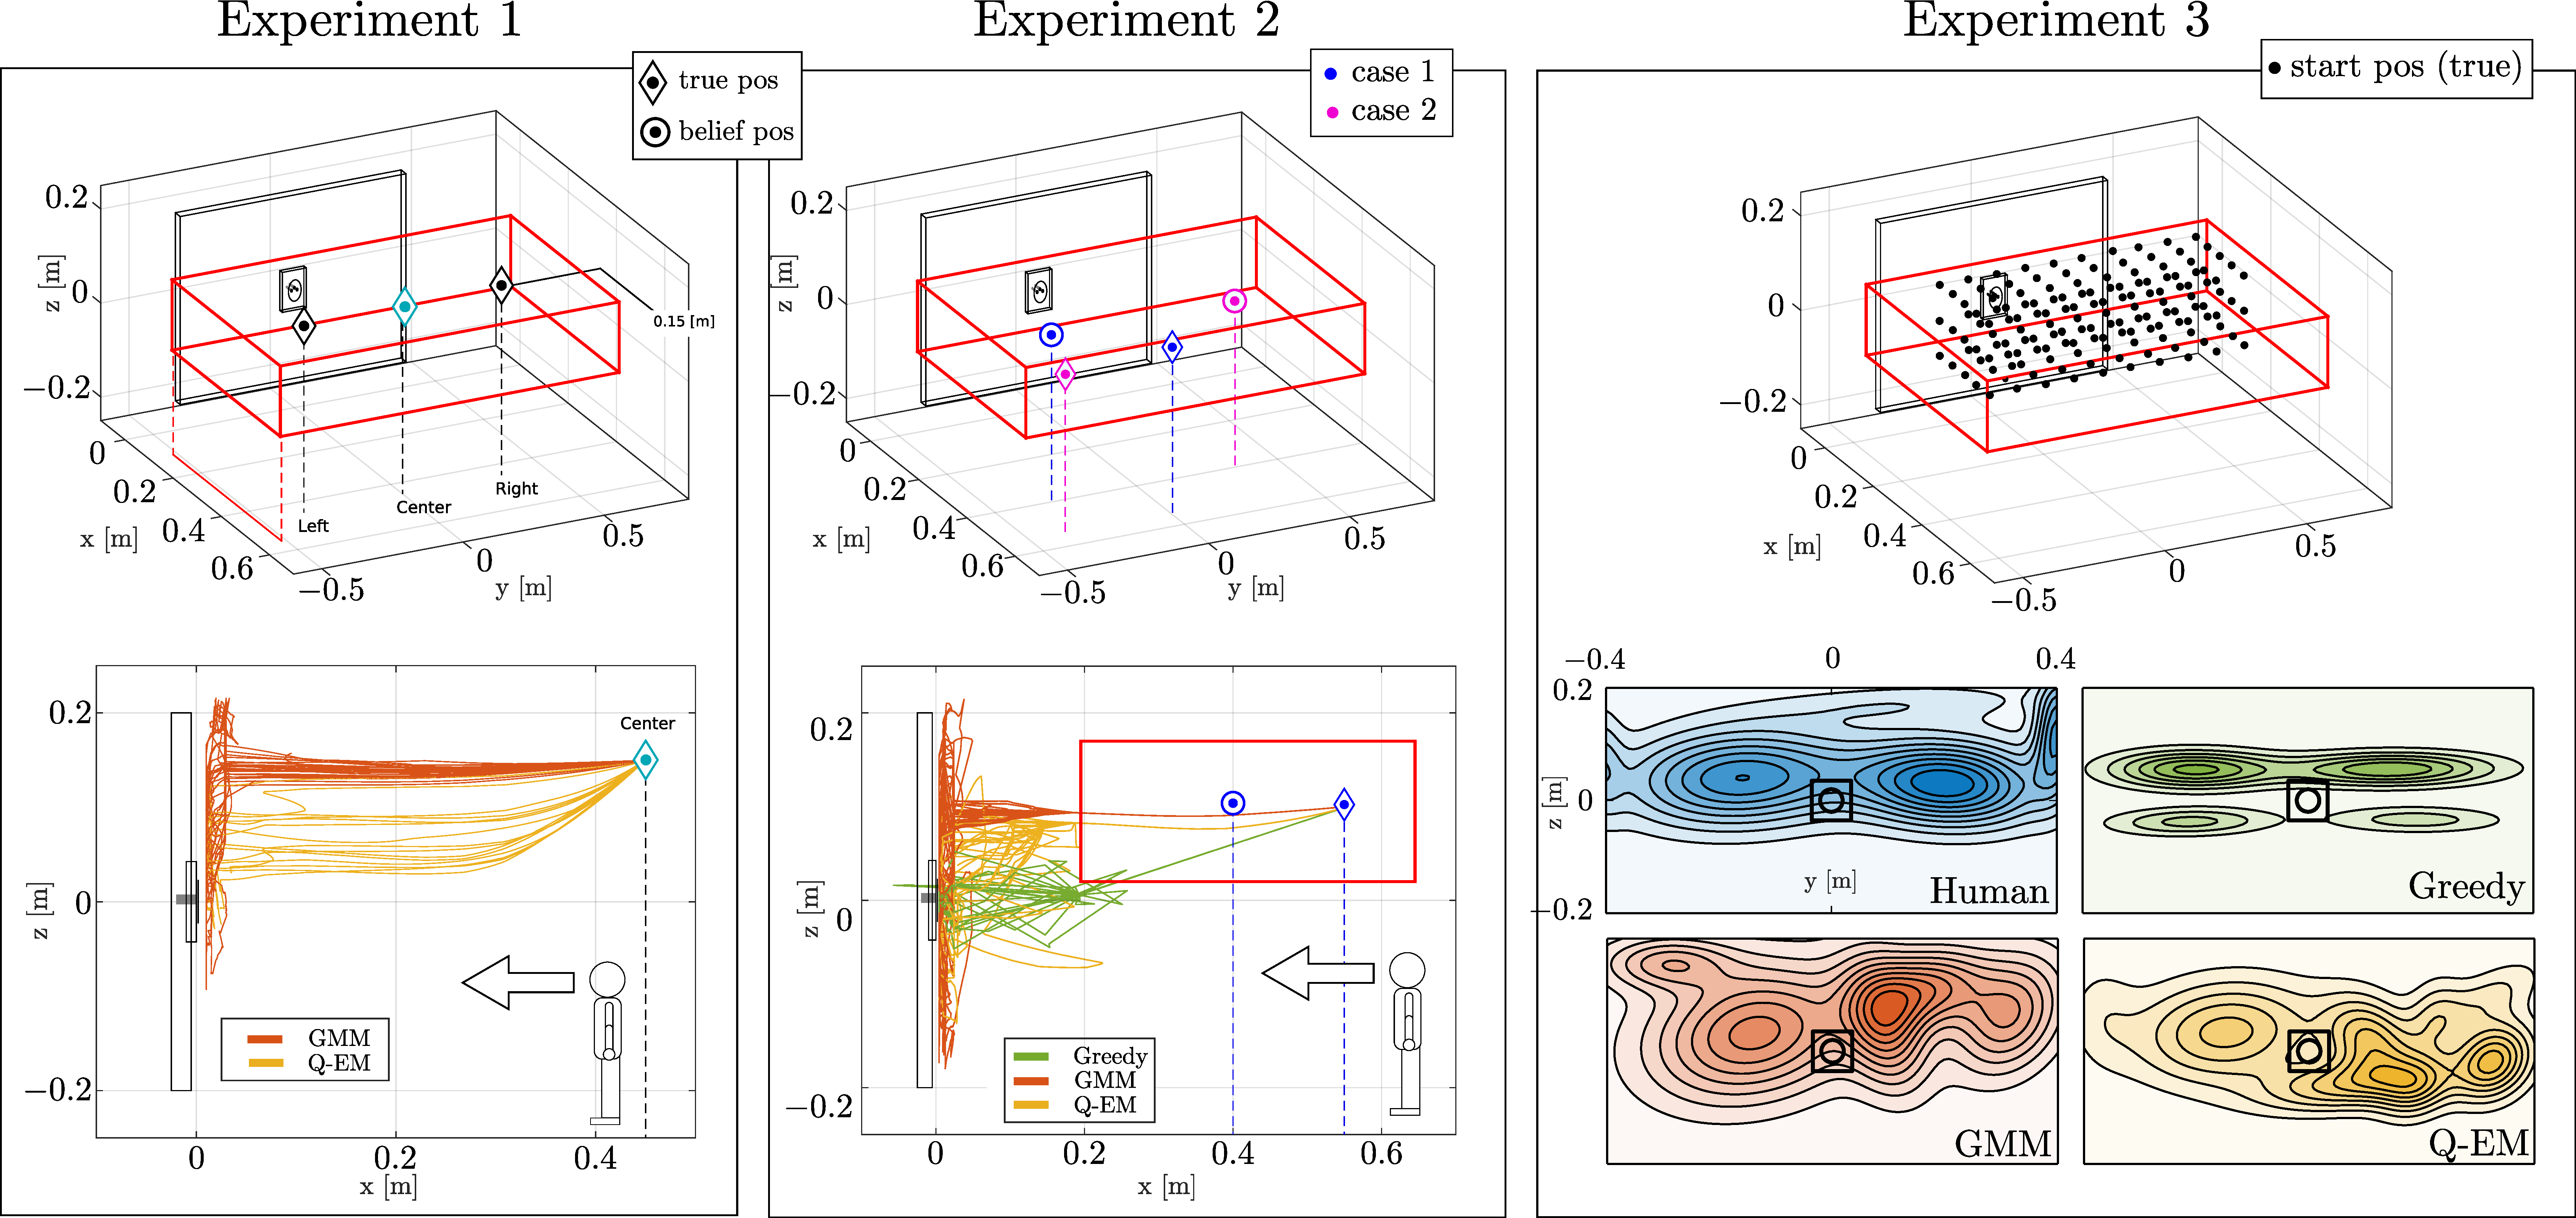
\includegraphics[width=\textwidth]{./ch4-PiH/Figures/Results1/Experiment_final_v2.pdf}
    \caption{Three simulated search experiments. \textbf{Experiment 1:} Three start positions are considered: \textit{Left}, \textit{Center} and
     \textit{Right} in which the triangles depict true position of the end-effector. The red cube illustrates the extent of the uncertainty. 
     In the second row of Experiment 1, we illustrate the trajectories of both the GMM (orange) and Q-EM (yellow) policies. For each start condition 
     a total of 25 searches were performed for each search policy. 
     \textbf{Experiment 2:} Two cases are considered: \textit{Case 1} blue, the initial belief state (circle) is fixed facing 
     the left edge of the wall and the true location (diamond) is facing the socket.
     \textit{Case 2} pink, the initial belief state (circle) is fixed to the right facing the edge of the wall and the 
     true location is the left edge of the wall. In the second row, the trajectories are plotted for \textit{Case 1}.
     \textbf{Experiment 3:} A 150 start locations are deterministically generated from a 
     grid in the start area. In the second row, we plot the distribution of the areas visited by the true position during the search.}
    \label{fig:box_exp_sim}
\end{figure}

We evaluate the performance of the three experiments in terms of the trajectories and their distribution in reaching 
the edge of the socket. 

We can see a clear difference between the trajectories generated by the GMM and Q-EM policies in Experiment 1, 
see Figure \ref{fig:box_exp_sim} \textit{Experiment 1, second row}. The orange GMM policy trajectories 
go straight towards the wall, whilst the yellow Q-EM policy trajectories drop in height which results in the trajectories being closer to the socket. 
The same effect can be seen in Experiment 2 (\textit{second row}). The Q-EM trajectories follow a downward trend towards the location of the socket. 
The gradient is less due to the initial starting condition being lower than in Experiment 1. 

The trajectories of the Greedy policy depend on the chosen believed location (most likely state of the PMF). In the 
second experiment there is no variance in the Greedy's trajectories until it reaches the edge of the red square. 
Where the branching occurs as the believed location is disqualified. This happens as  
no sensation is registered when the believed location reaches the wall as the true location is behind the believed location, see 
Figure \ref{fig:box_exp_sim}, \textit{Experiment 2, second row}.

In Figure \ref{fig:box_exp_sim} \textit{Experiment 3, second row}, both Human and GMM distributions of
searched locations are similar. They cover the upper region of the wall and top corners, to 
some extent. These distributions are not identical for two reasons. The first is that the learning of the GMM is a 
local optimisation which is dependent on initialisation and number of parameters. The second reason is that 
the synthesis of trajectories from the GMM is a stochastic process. 

The distribution of the searched locations of the Q-EM policy is centred around the origin of the $z$-axis,
see Figure \ref{fig:box_exp_sim}  \textit{Experiment 3, second row}. 
The uncertainty is predominantly located in the $x$ and $y$-axis. The Q-EM policy takes this uncertainty 
into consideration by restraining the search to the $y$-axis regardless of the starting position. The uncertainty 
is reduced whilst remaining in the vicinity of the socket. 
The Greedy's policy search distribution is multi-modal and centred around the $z$-axis where the modes are above 
and below the socket. This shows that the Greedy policy acts according to the most likely state 
which changes from left to right of the socket, because of motion noise, resulting in left-right 
movements and little displacement. As a result the Greedy policy spends more time at these modes.

In Figure \ref{fig:first_contact} (\textit{Top-left}), we illustrate the distribution of the first contact with the wall 
during Experiment 1 for the \textit{Center} initial conditions. The distribution of the first contact of the Greedy method is uniform across 
the entire $y$-axis of the wall. 
It does not take into account the variance of the uncertainty. In contrast, the GMM policy remains centred with respect to the starting position and the Q-EM is even closer to the socket and 
there is much less variance in the location of the first contact.

\begin{figure}
  \centering
   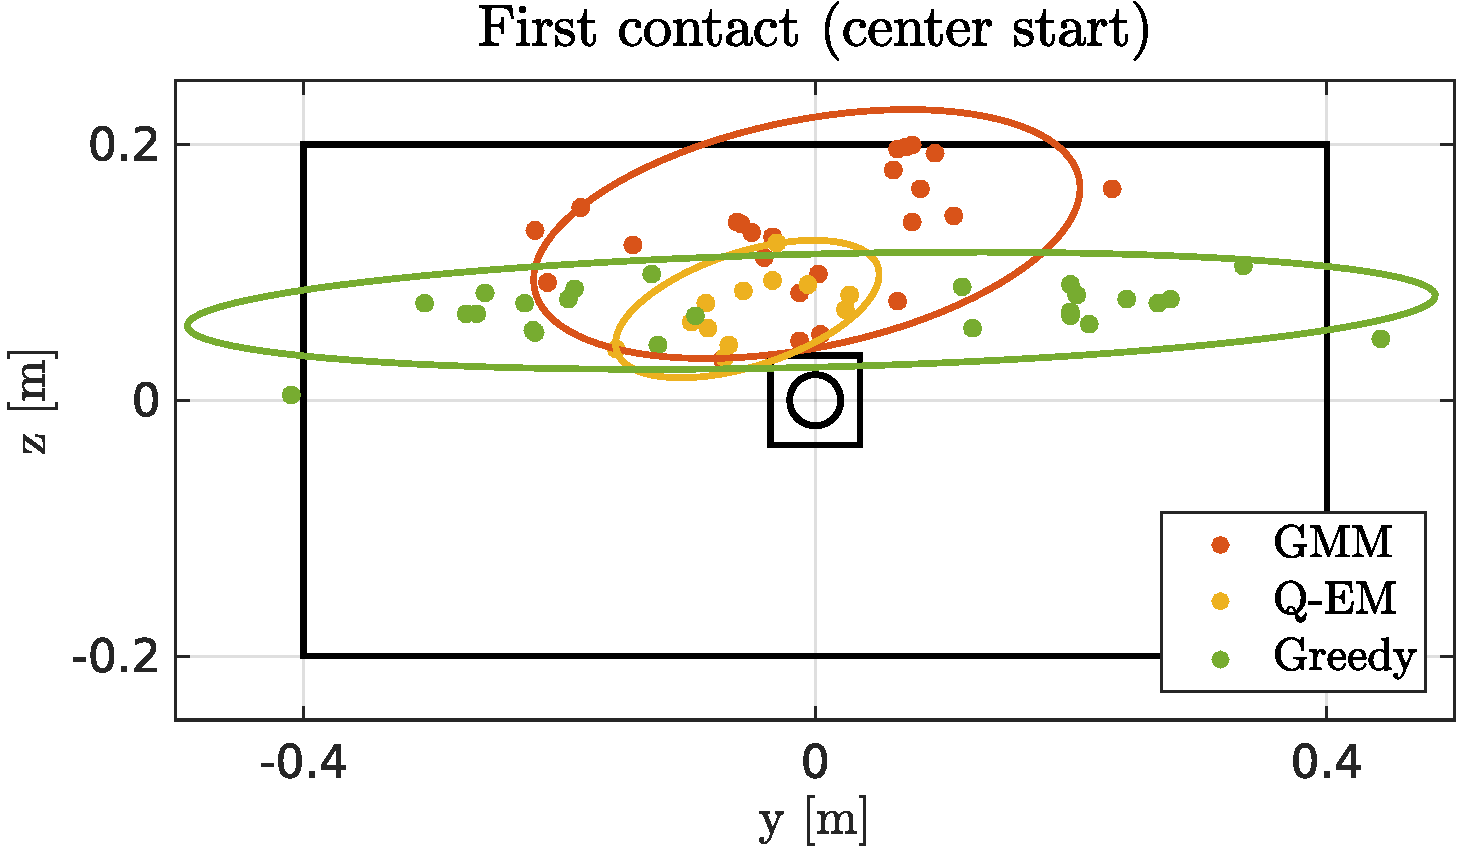
\includegraphics[width=0.45\textwidth]{./ch4-PiH/Figures/Results1/first_contact_center.pdf}
   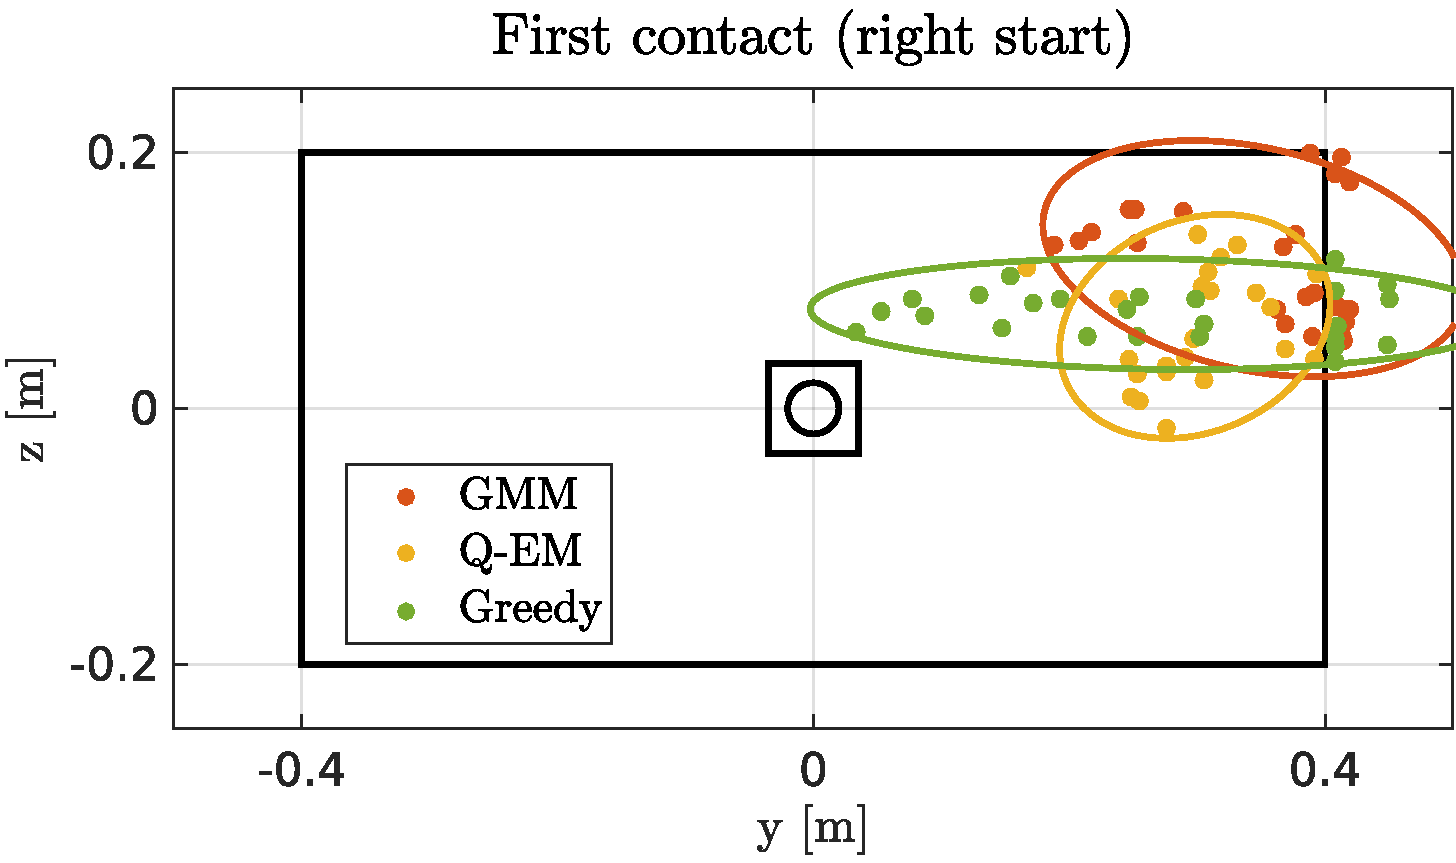
\includegraphics[width=0.45\textwidth]{./ch4-PiH/Figures/Results1/first_contact_right.pdf}
   \caption{First contact with the wall, during experiment 1. (a) Contact distribution for initial condition ``Center'' . (b) 
   Contact distribution for initial condition was ``Right''. The ellipses correspond to two standard deviations of a fitted Gaussian 
   function.}
   \label{fig:first_contact}
\end{figure}

\subsection{Distance taken to reach socket's edge (Quantitative)}

In Figure \ref{fig:three_searches} we illustrate the quantitative results of the distance taken 
to reach the socket for all three experiments. In \textbf{Experiment 1}, for the \textit{Center} initial condition,
the Q-EM policy travels a far less than the other search policies. Considering that the initial position of the search is 
0.45 [m] away from the wall, the Q-EM policy finds the socket very quickly once contact has been established with the wall. 
For the \textit{Right} and \textit{Left} starting conditions both the GMM and Q-EM policies travel less distance to reach the socket, with a 
smaller variance when compared with the Greedy search policy.

In \textbf{Experiment 2}, the Q-EM search policy is the most efficient. For \textit{Case 1} of Experiment 2, the initial most 
likely state is fixed to the left and the true position is facing the socket. Because the belief is chosen to be 
to the left, upon contact with the wall the policy takes a left action since it is more likely to result in a localisation, given 
the left edge of the wall is within close proximity. 
This on average results in an exploration in the upper left area of the wall, which explains why \textit{Case 1} does worse than 
for the \textit{Center} initial condition of Experiment 1. Less distance is taken to find the socket in Case 2, than it does for Case 1, 
Figure \ref{fig:three_searches} (b). The reason for the improvement over Case 1, is that in \textit{Case 2}. The true location of 
the end-effector is close to an edge which is an informative feature and results in a much faster localisation.

From \textbf{Experiment 3}, Figure \ref{fig:three_searches} (c), it is clear that there is less variation in the distance travelled to find the socket's 
edge amongst the three search policies than it is for the human teachers. All search policies are better than the human teachers 
with the exception of group B\textsuperscript{*}. The Q-EM policy is however still the best. 

\begin{figure}
 \centering
   \subfigure[]{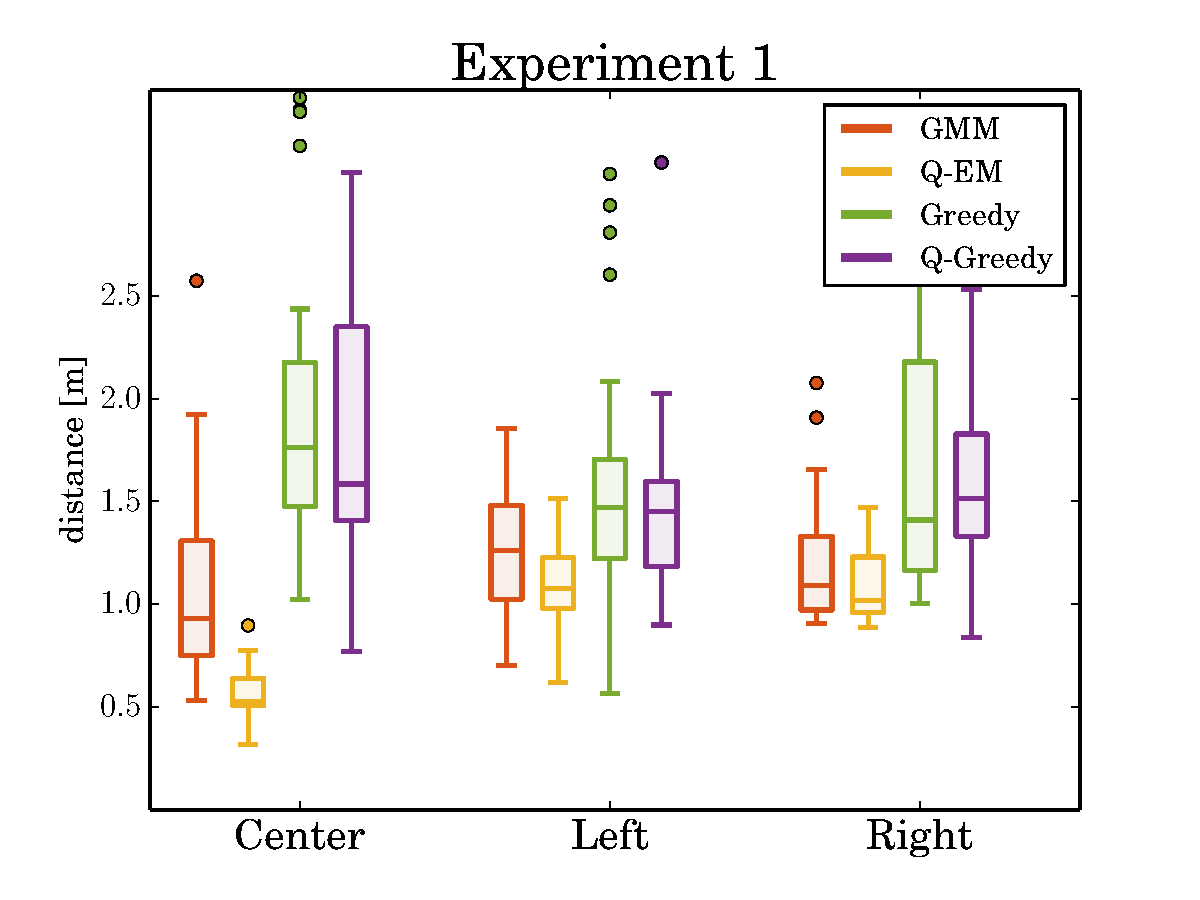
\includegraphics[width=0.33\textwidth]{./ch4-PiH/Figures/Results1/experiment1.pdf}}\hfill
   \subfigure[]{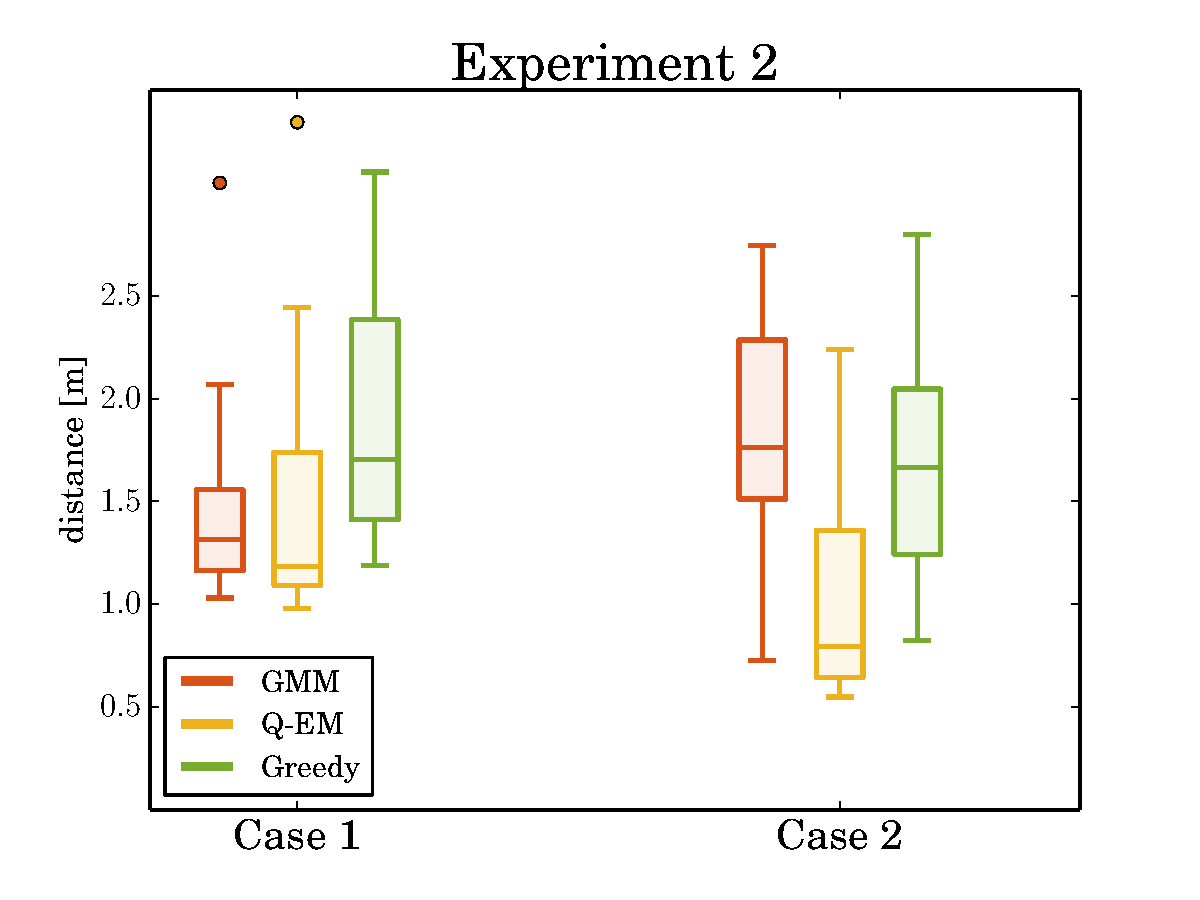
\includegraphics[width=0.33\textwidth]{./ch4-PiH/Figures/Results1/experiment2.pdf}}\hfill
   \subfigure[]{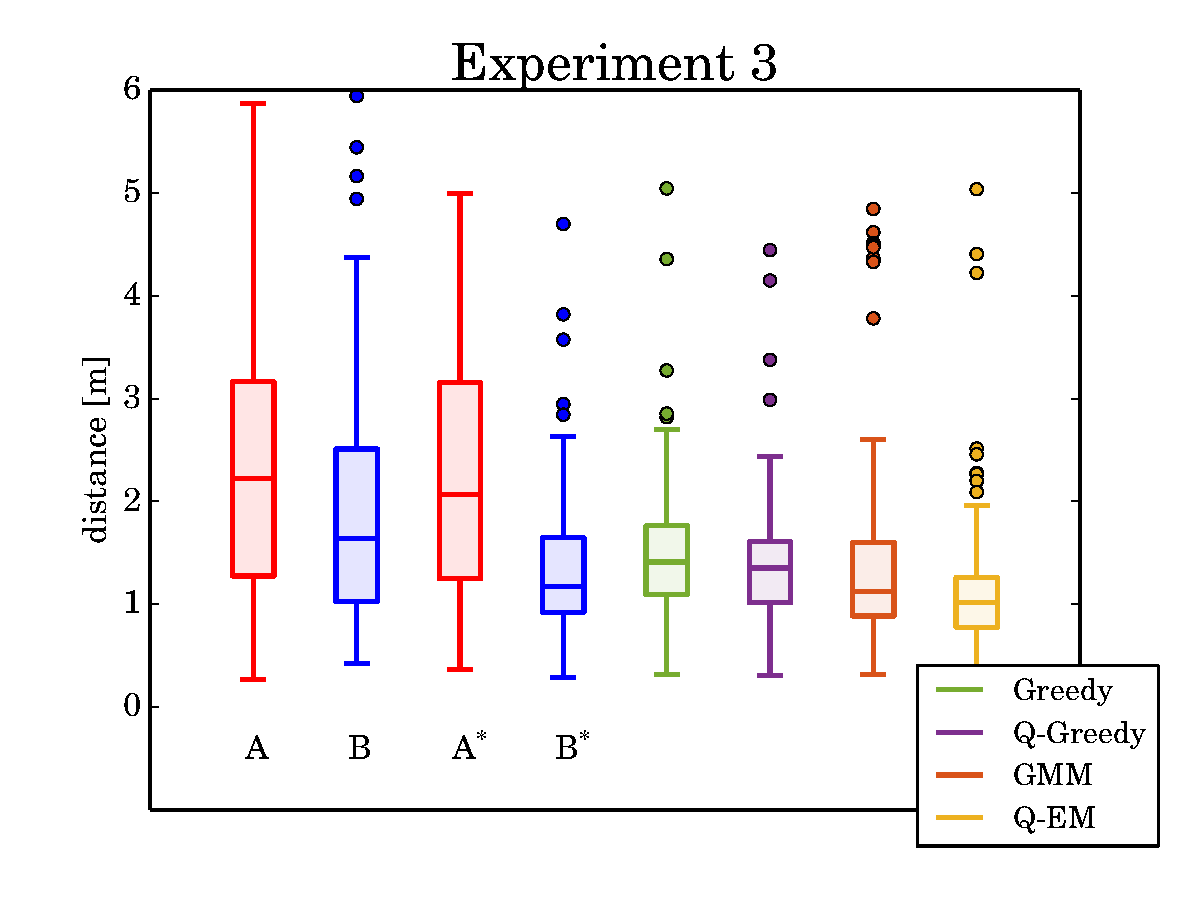
\includegraphics[width=0.33\textwidth]{./ch4-PiH/Figures/Results1/experiment3_plot2.pdf}}
   \caption{Distance travelled until the socket's edge is reached. (a) Three groups correspond to the initial conditions: Center, Left and Right
   depicted in Figure \ref{fig:three_searches}, \textit{top left}. The Q-EM method is always better than the other methods, in terms of distance. (b)
   Results of the two initial conditions depicted in Figure \ref{fig:three_searches}, \textit{top middle}, both the true position and most likely state is
   fixed. The Q-EM method always improves on the GMM. (c) Results corresponding to Experiment 3, Figure \ref{fig:three_searches}, \textit{top right}.
   Again the Q-EM method is better, but at a less significant level.}
   \label{fig:three_searches}
\end{figure}


We have shown that under three different experimental settings the Q-EM algorithm is predominantly the best in terms of distance taken 
to localise the socket. The GMM policy learned solely form the data provided by the human teachers also performs well in comparison to  
the human teachers and Greedy policy. There is however a critical assumption we made such to be able to use our (RL-)PbD-POMDP approach. This \textbf{assumption} 
is that a human teacher is proficient in accomplishing the task. If a teacher is not able to accomplish the task in a repetitive and consitent way such that 
a search patter can be encoded by the GMM, the learned policy will perform poorly. Next we evaluate the validity of 
this assumption and the importance of the training data provided by the human teachers.
% 
\subsection{Importance of data}

We perform two tests to evaluate the importance of the teachers training data for learning a search policy. We first take the 
worst two teachers in terms of distance taken to find the socket's edge and learn a GMM and Q-EM policy from their 
demonstrations separately. In this way we can evaluate if it is possible to learn a successful policy given 
a few bad demonstrations (15 training trajectories for each policy). Our second evaluation consists of using a noisy 
explorative Greedy policy as a teacher to gather demonstrations to learn policy, which we call Q-Greedy. 

In Figure \ref{fig:subj_5_traj}, 6 trajectories of Teacher \# 5 are illustrated. The human teacher preferred to first 
localise himself at the top of the wall before proceeding either to a corner or directly towards the socket. Once localised, the teacher 
would reposition himself in front of the socket and try to achieve an insertion. This behaviour was not expected 
since by loosing contact with the table, the human subject has no more sensory feedback which is necessary 
to maintain an accurate position estimate.

\begin{figure}
 \centering
    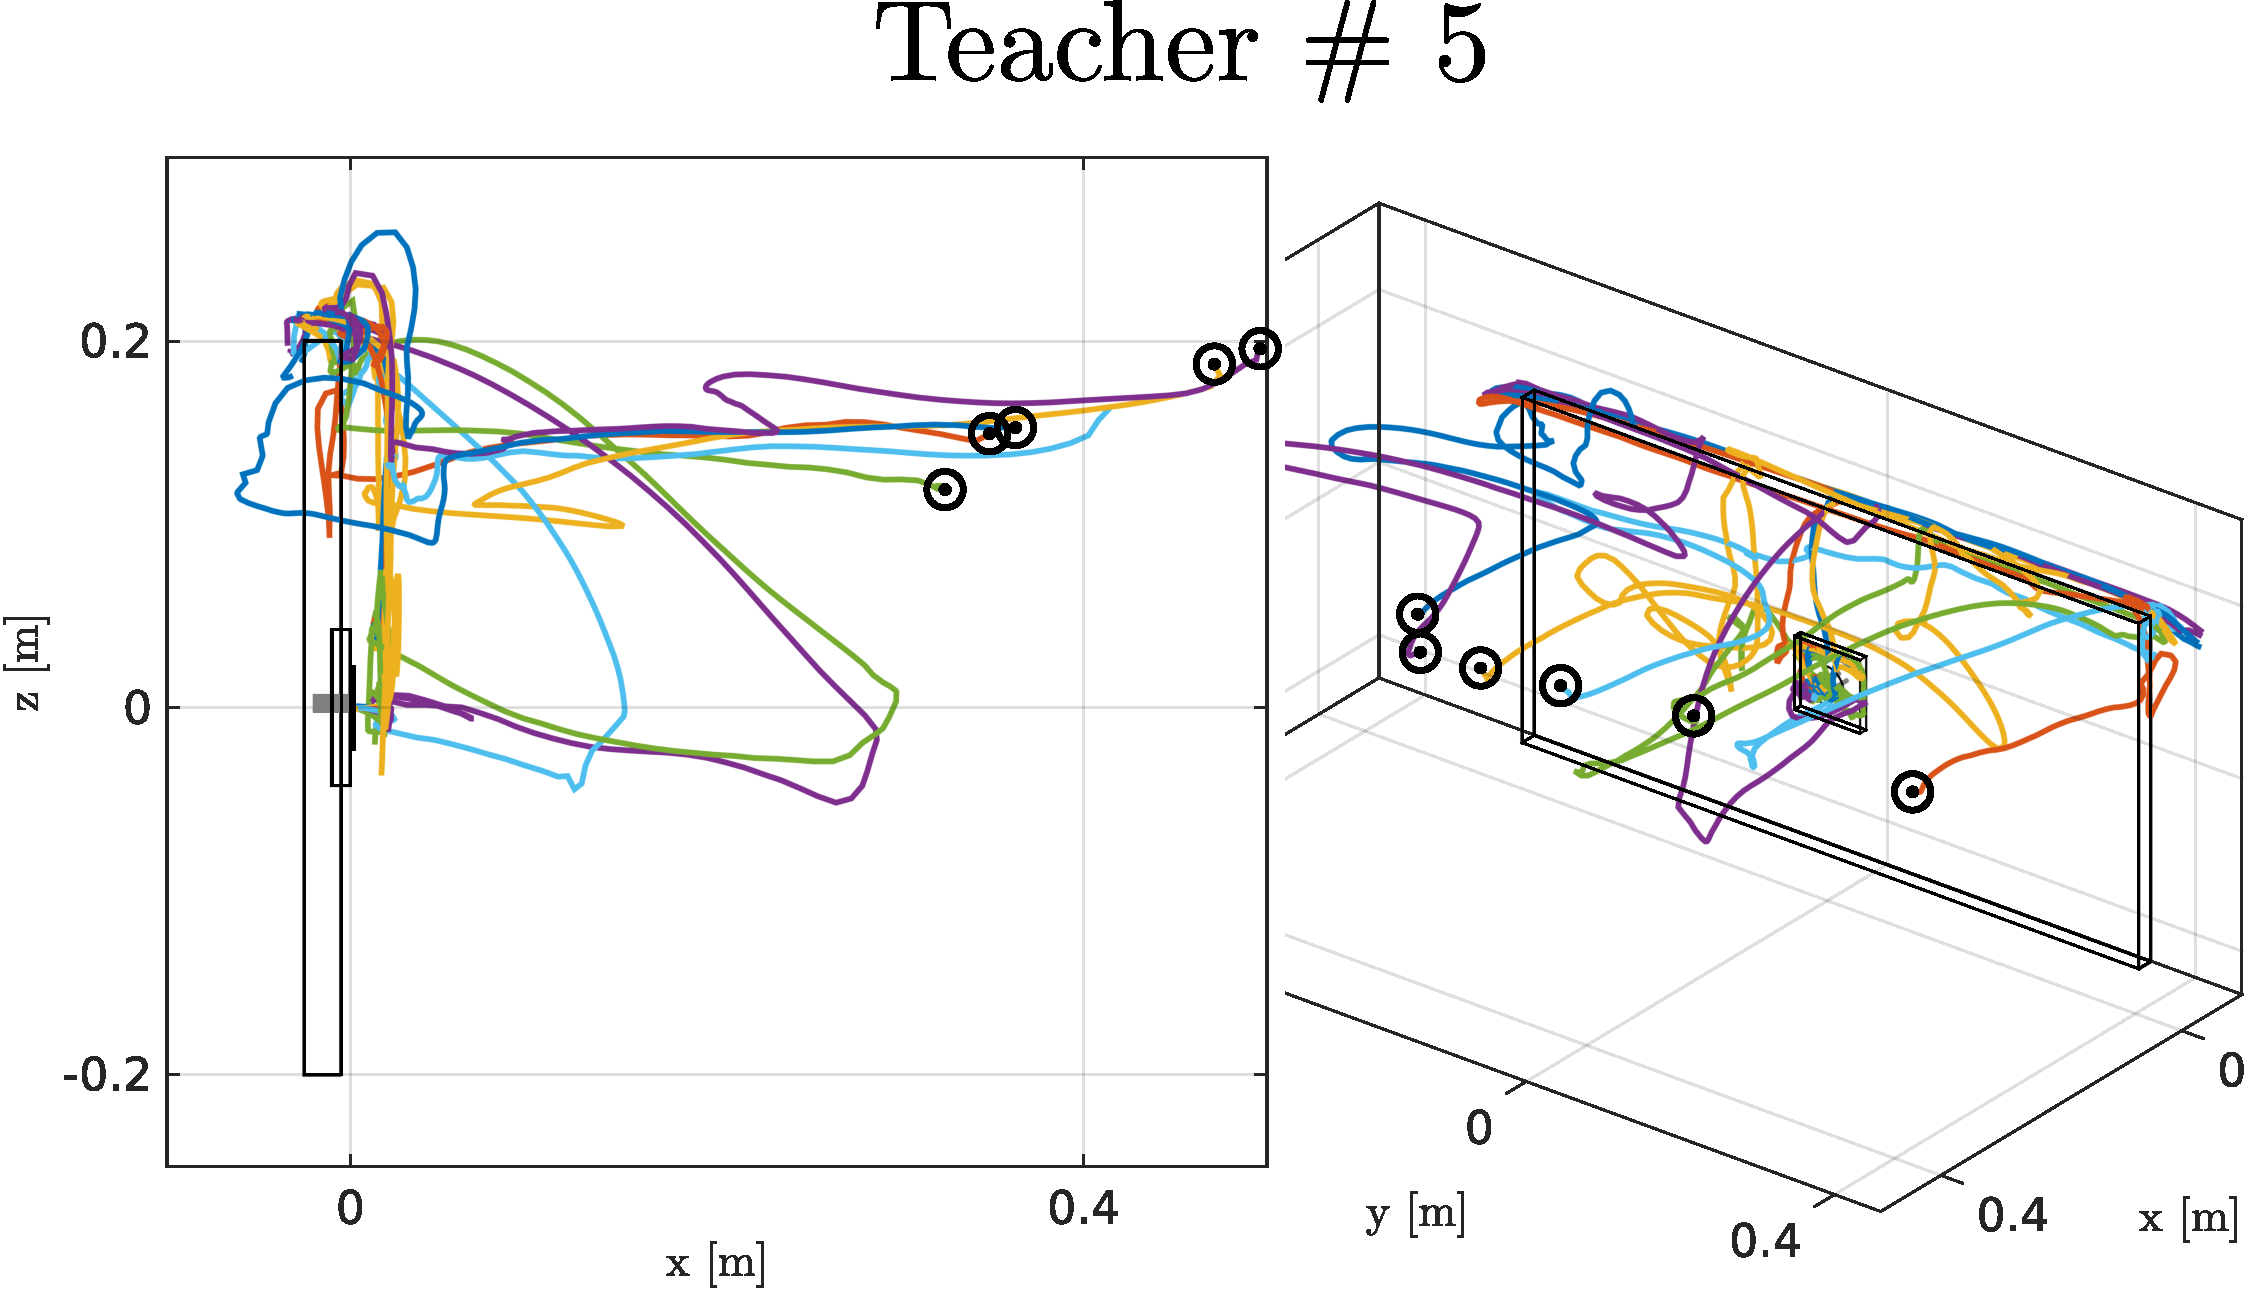
\includegraphics[width=\textwidth]{./ch4-PiH/Figures/Results1/experiment4/subject5.pdf}
%    \subfigure[]{\includegraphics[width=0.45\textwidth]{./Figures/Results1/experiment4/value_subj_5.pdf}}
%    \subfigure[]{\includegraphics[width=0.445\textwidth]{./Figures/Results1/experiment4/experiment4.pdf}}
    \caption{Original demonstrations of teacher \# 5. The teacher demonstrates a preference
    to first go to the top of the wall and then leaves contact with the table to position himself in front of the socket, before trying to 
    to find it}
    \label{fig:subj_5_traj}
 \end{figure}
 
\begin{figure}
 \centering
 \includegraphics[width=0.8\textwidth]{./ch4-PiH/Figures/Results1/experiment4/value_subj_5.pdf}
 \caption{Value function learned from the 15 demonstrations of teacher \#5.}
 \label{fig:value_function_subj_5}
\end{figure}
 
 \begin{figure}
    \centering
    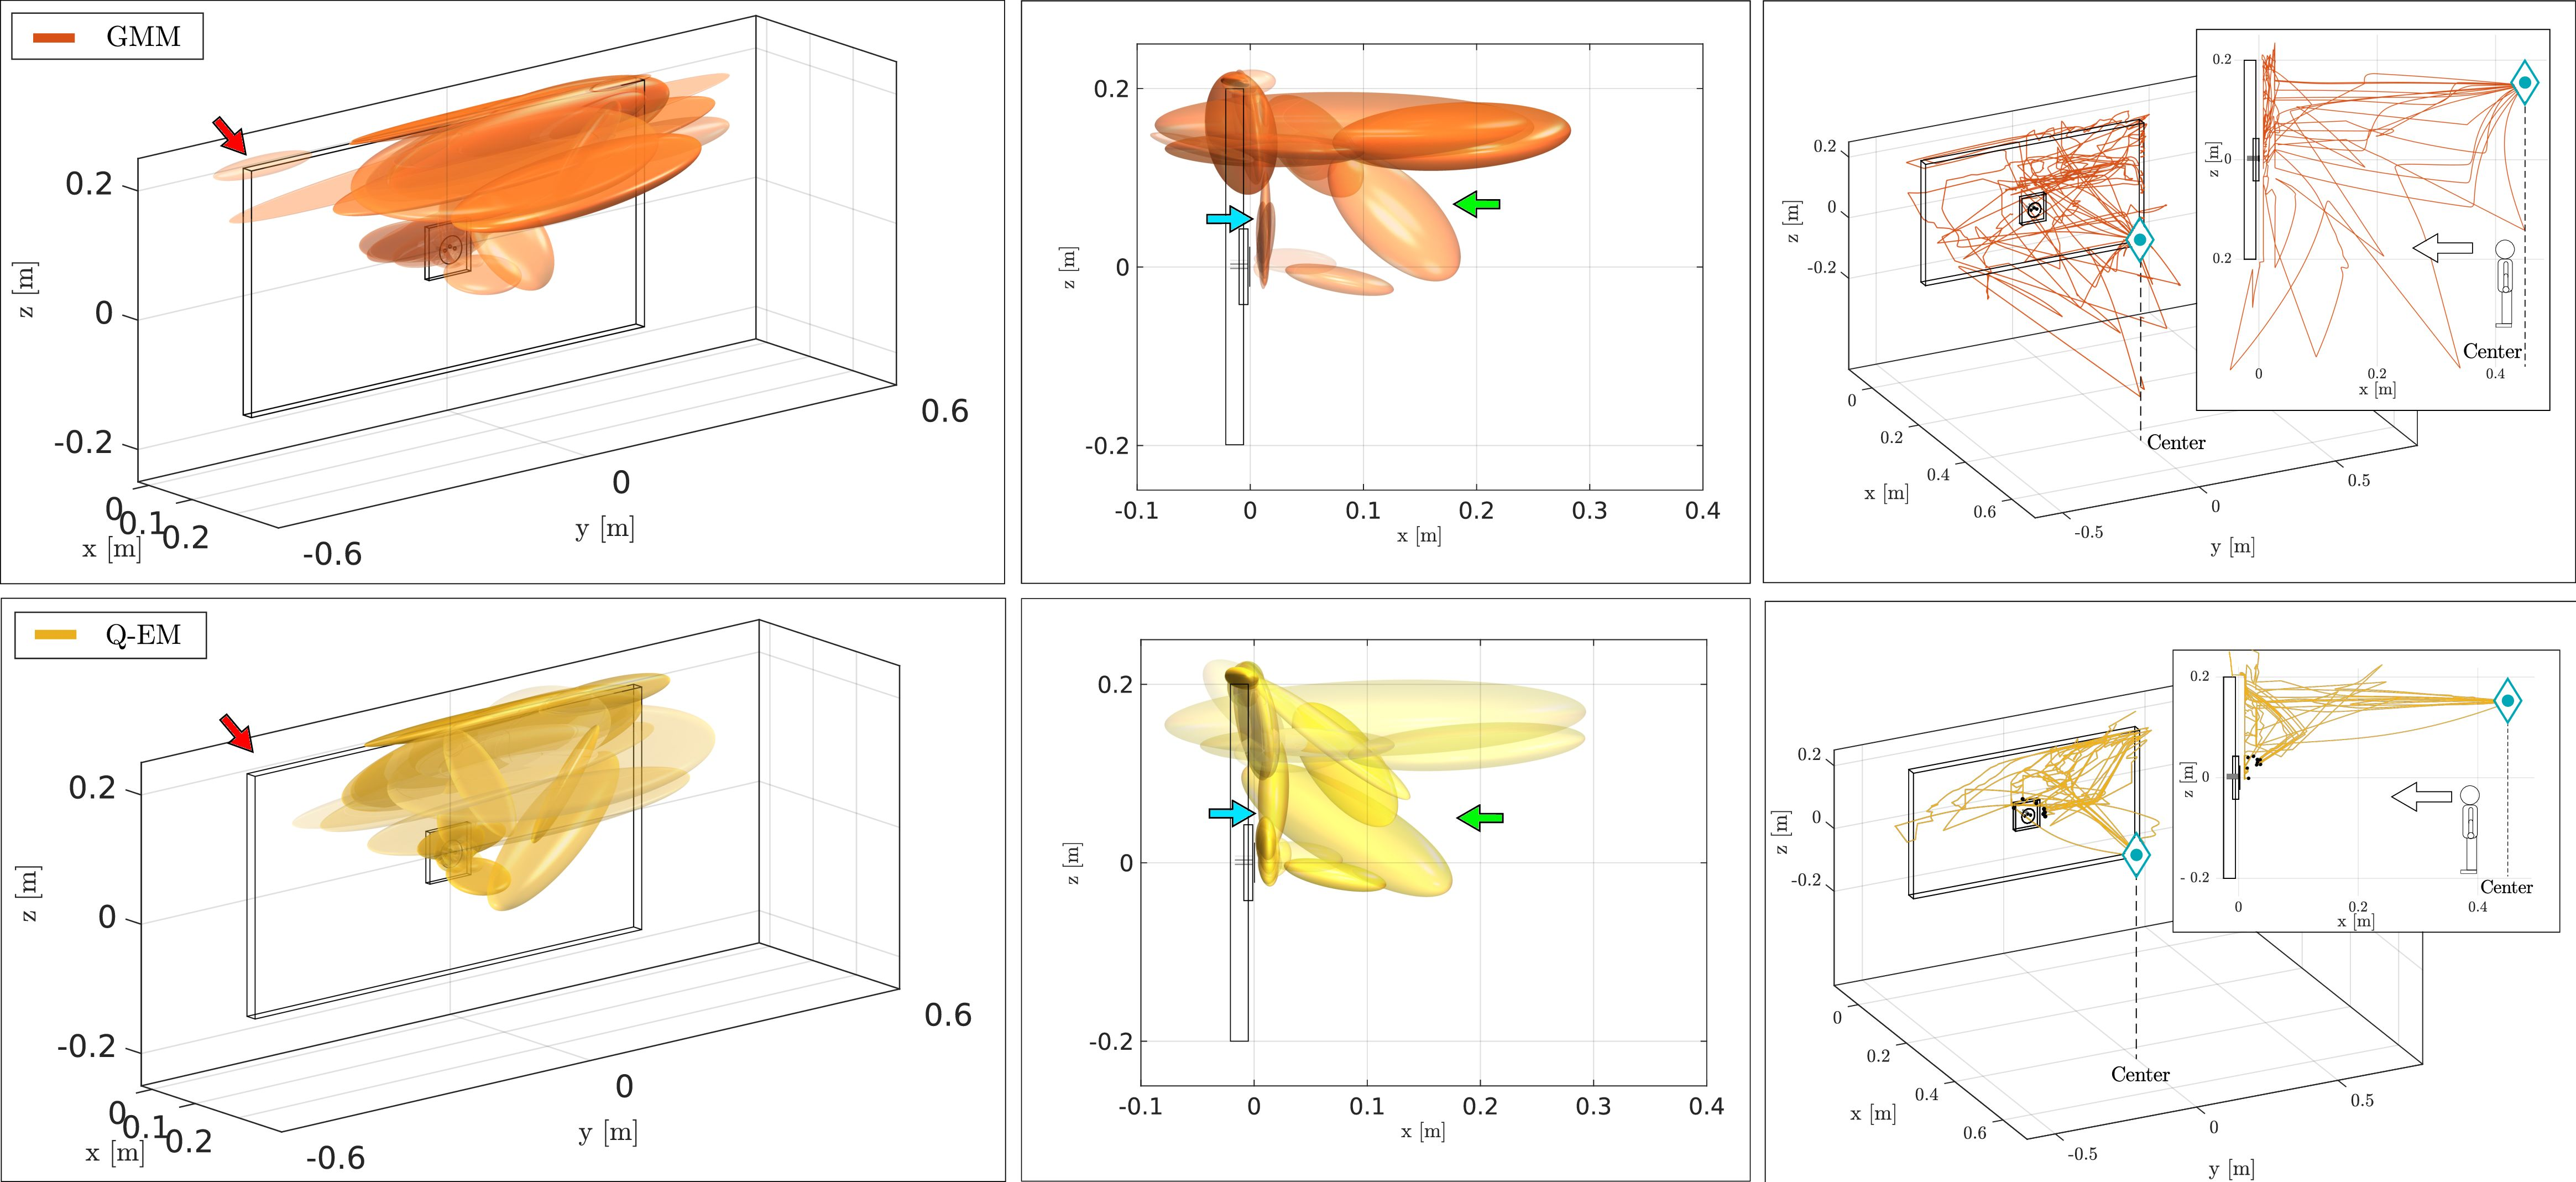
\includegraphics[width=\textwidth]{./ch4-PiH/Figures/Results1/experiment4/gmm.pdf}
    \caption{Marginalised Gaussian Mixture parameters of the GMM and Q-EM learned from the demonstrations of teacher \#5. 
    The transparency of the Gaussian functions illustrated is proportional to their weight.
    \textit{Left column}: The Gaussian functions of the Q-EM have shifted from the left corner to the right, this is a result of the value function 
    being higher in the top right corner region, see Figure \ref{fig:value_function_subj_5}. \textit{Center column}:  The original data of the teacher 
    went quite fare back which results in a Gaussian function given a direction which moves away from the table (green arrow), whilst in the case
    of the Q-EM parameters this effect is reduced and moved closer towards the table.  We can also see from the two plots of the Q-EM parameters 
    that they then to follow the paths encoded by the value function.    
    \textit{Right column}: Rollouts of the policies learned from teacher \#5. We can see that trajectories from the GMM policy have not really 
    encoded a specific search patter, whilst the Q-EM policy gives much more consistent trajectories which seem to replicate to some extend 
    the pattern of making a jump (no contact with the table) from the top right corner to the socket's edge.}
    \label{fig:gmm_exp4}
\end{figure}
 
In Figure \ref{fig:value_function_subj_5}, the value function of the belief state learned from the data of teacher \# 5 is 
illustrated. The states with the highest values seem to create a path going from the socket towards the right edge of the wall. 
We proceed as before to learn a GMM policy from the raw data and a Q-EM policy in which the data points are weighted by 
the gradient of the value function. In Figure \ref{fig:gmm_exp4}, we illustrate the 
resulting Marginalised Gaussian Mixture parameters for both the GMM and Q-EM policies and we plot 25 rollouts of each policy starting at 
the \textit{Center} initial condition used in Experiment 1. We note that the trajectories of the GMM 
policy seams to have a lot of variance in contrast to the Q-EM policy. This is because there is too much variance amongst the 15 original demonstrations
given by the teacher. As a result to there is insufficient data such that a patter can encoded in the GMM model. In contrast the Q-EM find a 
pattern by combining multiple parts of the available data and as a result fewer data points are necessary to achieve a good policy. 
This effect is clear in Figure \ref{fig:experiment4_stats}, in which we evaluated the performance of the GMM and Q-EM algorithms 
under the same initial conditions used in Experiment 1. For all the conditions for both teacher \#5 and \#7 the Q-EM policy 
always does better than the GMM.

\begin{figure}
 \centering
 \includegraphics[width=0.8\textwidth]{./ch4-PiH/Figures/Results1/experiment4/experiment4.pdf}
 \caption{Results of a GMM and Q-EM policy under the same test conditions as Experiment 1. The Q-EM policy nearly always does much better than the GMM policy.}
 \label{fig:experiment4_stats}
\end{figure}

The second point we tested is whether we could use the Greedy policy as means of gathering demonstrations such to learn a value function and 
train a Q-Greedy policy. We used the Q-Greedy algorithm in combination with random perturbation applied to the Greedy velocity to act as 
simple exploration technique. We performed a 150 searches, which we terminated once the socket was found, and used these demonstrations to 
learn a value function and GMM policy which we refer to as Q-Greedy. In Figure \ref{fig:three_searches} the statistical results 
of the Q-Greedy policy are illustrated for Experiment 1 and 3. We see that there is no difference between the Greedy and Q-Greedy policy. 
Our exploration method is probably too simplistic to allow to discover meaningful search patterns. We could probably devise better 
search strategies which would result in good policy, but the point was to show that human behaviour does already have a usable trade-off 
between exploration and exploitation which can be used to learn a policy through our RL-PbD-POMDP framework.

\subsection{Generalisation}

An important aspect of a policy or any machine learning methodology is to be able to generalise. So fare we have trained and 
evaluated our policy in the same environment. To test the ability of our GMM policies to generalise to a new setting we changed 
the location of the socket to the upper right corner of the wall. The GMM was trained in the frame of reference of the socket and
when we translate the socket's location it also translates the policy. 

\begin{figure}
 \centering
    \subfigure[]{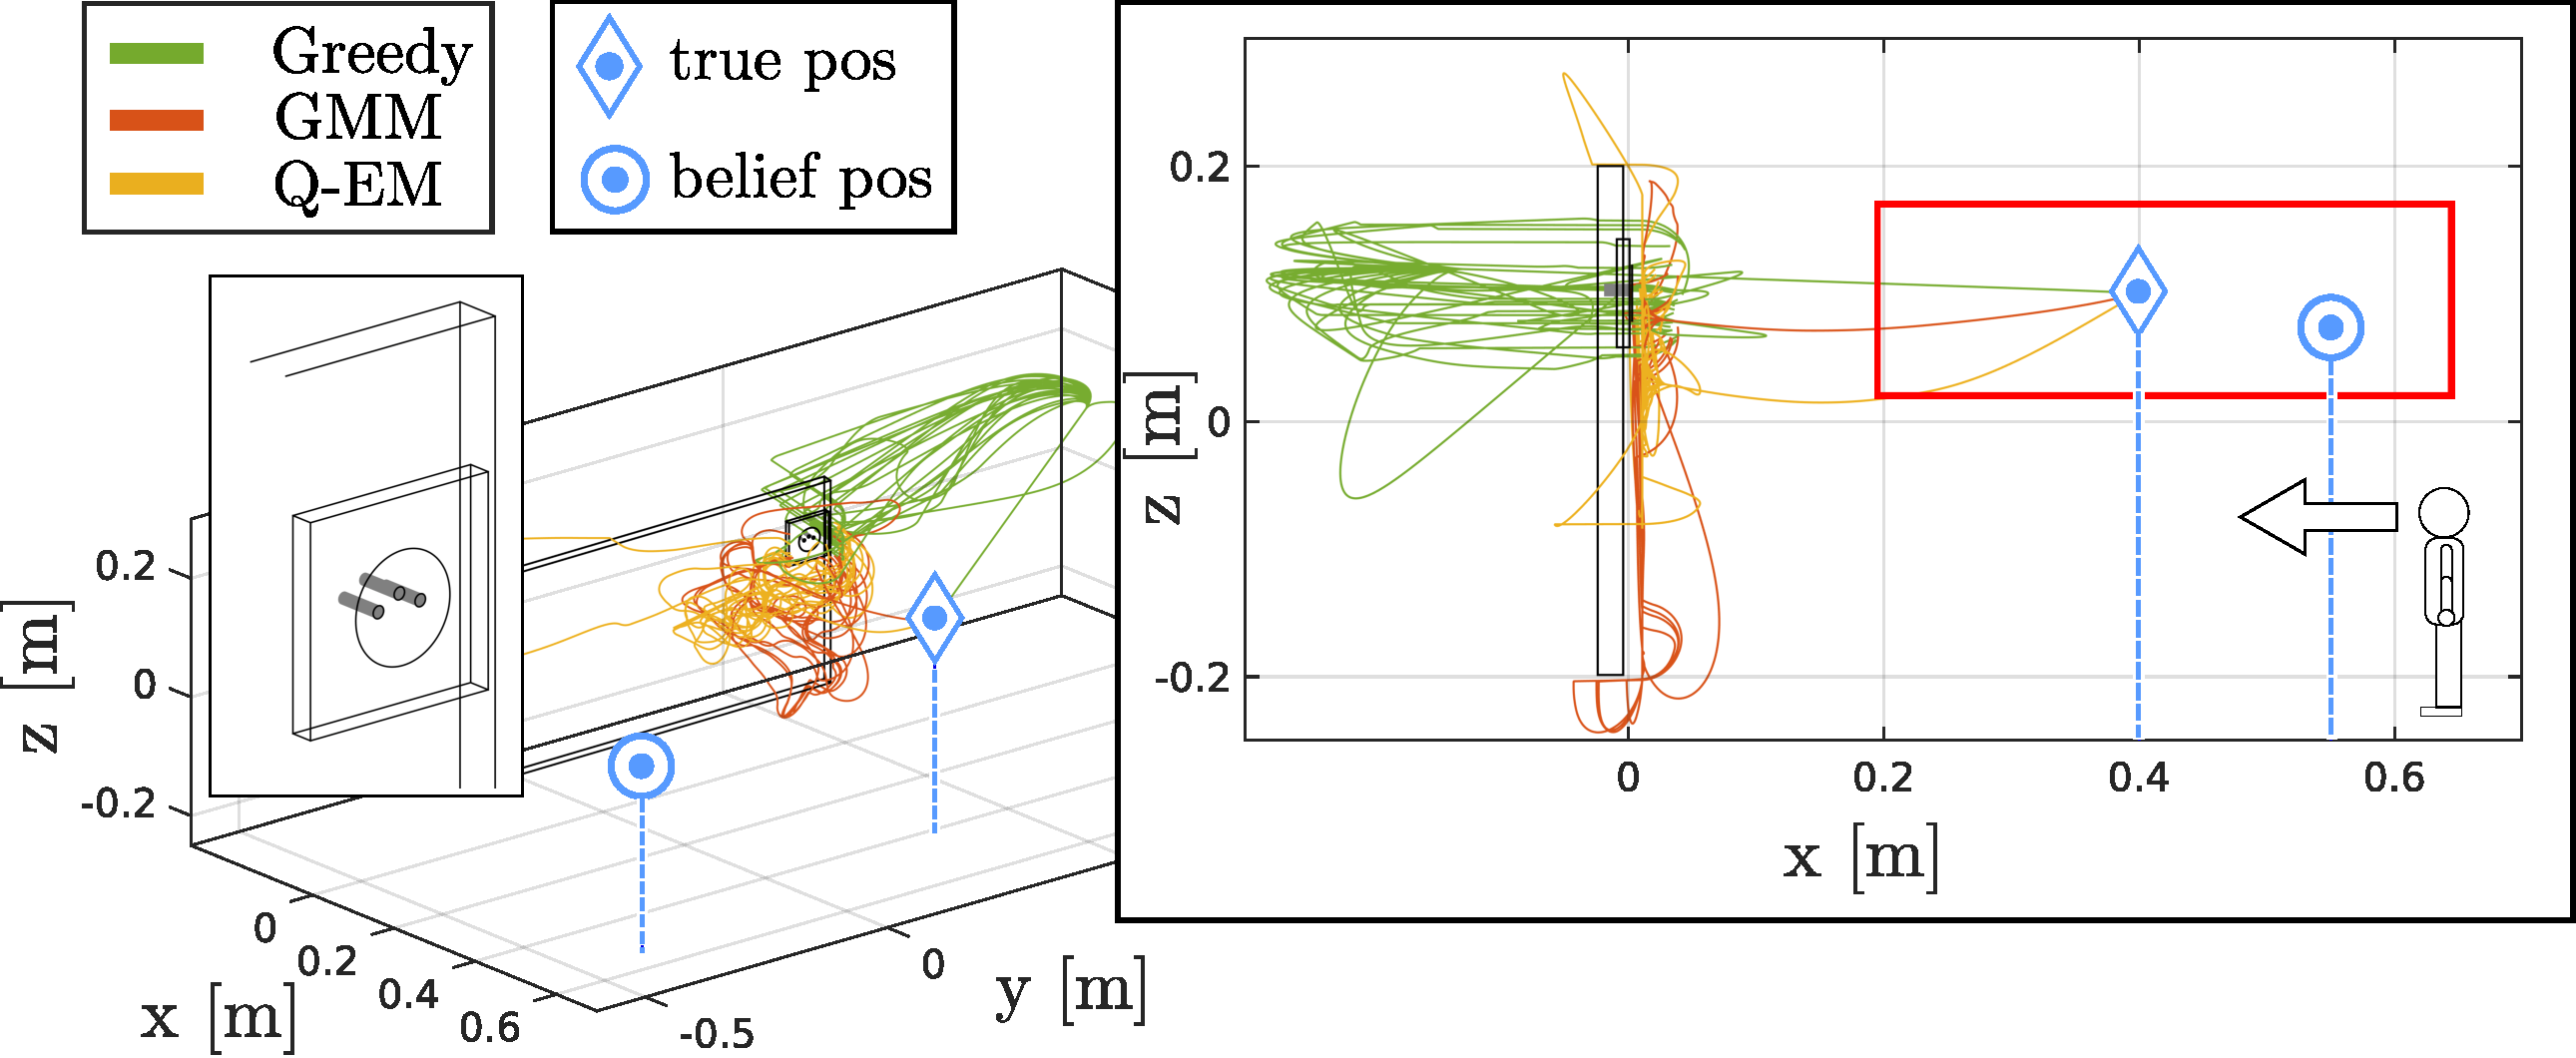
\includegraphics[width=\textwidth]{./ch4-PiH/Figures/Results1/experiment5/traj_experiment5.pdf}}
    \caption{Evaluation of generalisation. The socket is located in at the top right corner of the wall. We consider the 
    starting a Fixed starting location for both the true and most likely location of the end-effector. The red square depicts the 
    extend of the initial uncertainty, which is uniform. (b) Distance taken to reach the socket's edge. For the Fixed setup (see (a) for 
    the initial condition), both the Q-EM and GMM significantly outperform the Greedy. The other three conditions are the same as for 
    Experiment 1. }
    \label{fig:experiment5_traj}
\end{figure}

\begin{figure}
 \centering
    \subfigure[]{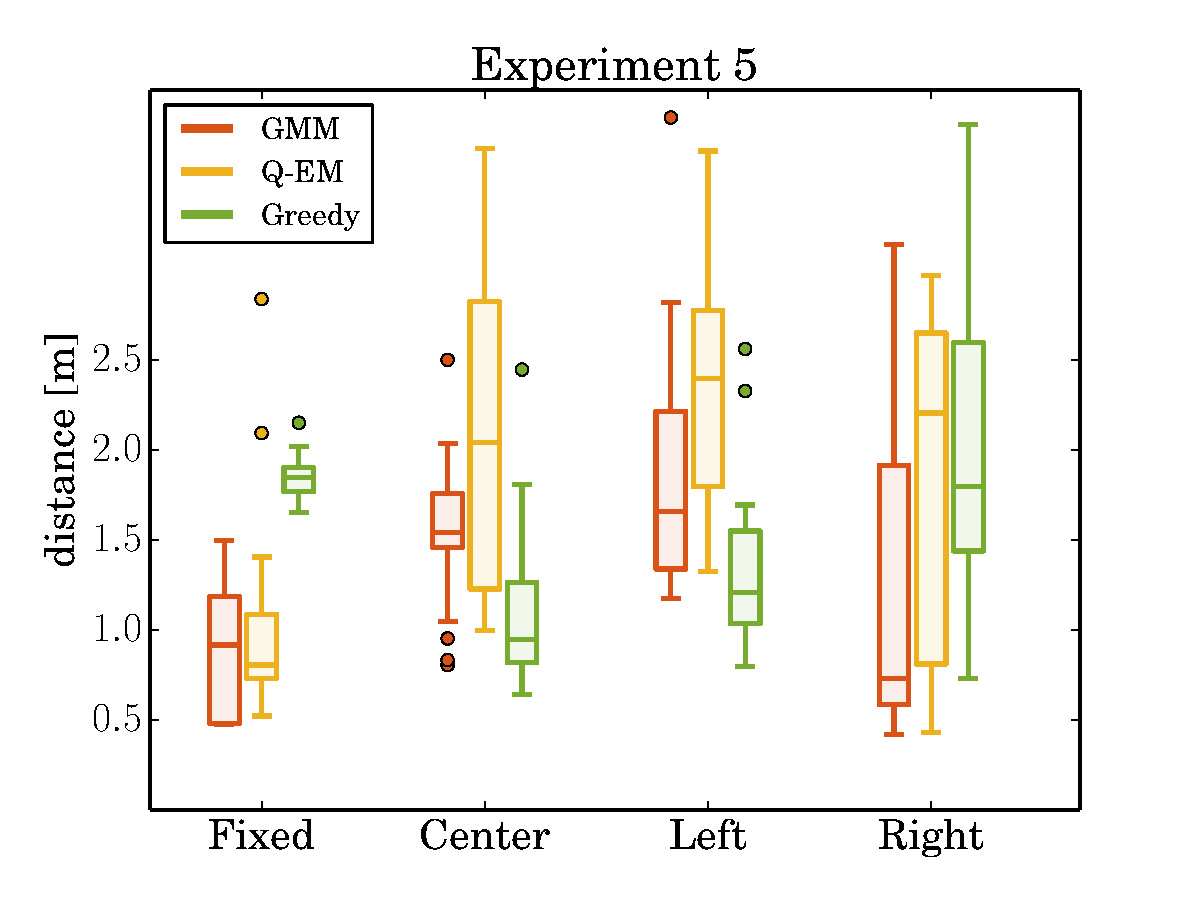
\includegraphics[width=0.8\textwidth]{./ch4-PiH/Figures/Results1/experiment5/experiment5.pdf}}
    \caption{Distance taken to reach the socket's edge. For the Fixed setup (see Figure \ref{fig:experiment5_traj}) for 
    the initial condition), both the Q-EM and GMM significantly outperform the Greedy. The other three conditions are the same as for 
    Experiment 1. }
    \label{fig:experiment5_stats}
\end{figure}

To evaluate the generalisation of our learned policy we use the same initial conditions of Experiment 1 with an additional 
new configuration named \textit{Fixed}, in which both the true and believed location are fixed, 
see Figure \ref{fig:experiment5_traj}; blue triangle and circle. In Figure \ref{fig:experiment5_traj}, we illustrate the trajectories 
of the three search policies for the \textit{Fixed} initial condition. The Greedy policy moves in a straight line towards the top
right corner of the table. Because the true position is to the right it takes longer for the Greedy policy to find the wall 
in contrast to both the GMM and Q-EM policies. From the statistical results shown in Figure \ref{fig:experiment5_stats} we can see
that for the \textit{Fixed} and \textit{Right} initial condition, which are similar, both GMM and Q-EM are better. However, for 
the \textit{Center} and \textit{Left} initial condition this is no longer the case. 
The reason that the Greedy method is better under this condition is that the socket is close to informative features, since it 
is located close to the edges of the wall. Once the end-effector has entered in contact with the wall the actions of the Greedy 
policy always result in a decrease of uncertainty, which was not the case when the socket was located in the center of wall. 
This is why both in the \textit{Fixed} and \textit{Right} initial condition the Greedy method does worse, because it takes a longer
time to find the wall.

The GMM based policies are still able to generalise under different socket locations. In general, as the socket's location is moved 
further from the original frame of reference, in which it was learned, the more likely the search quality will degrade. We 
chose the upper right corner since it is the furthest point from the origin and the GMM and Q-EM policies where still able to find 
the socket. The policy will always be able to find the socket once it has localised itself, this is can be seen from the vector field 
of the policy, see Figure \ref{fig:policy_vf}, when the entropy is low. In this case the policy acts like a point attractor.

\subsection{Distance taken to connect the peg to the socket}
% Real socket experiment.
% Show initial condition setup with belief. (the experiment)
We evaluated in simulation the performance of the search policies in localising the socket's edge. In this
section we evaluate the distance taken for the policies and humans to establish a connection, after the socket 
has been found. We start measuring the distance 
from the point that the peg enters in contact with the socket's edge until the peg is connected to the socket. All the following evaluations are done 
on a KUKA LWR4 robot. The robot's end-effector is equipped with a peg holder on which is attached a force-torque sensor, 
the same we used during the demonstration of the human teachers. In this way both the teacher and robot apprentice share 
the same sensory interface.

We chose to have the robot's peg end-effector located to the right of the socket and a belief spread uniformly 
vertically along the z-axis, see Figure \ref{fig:real_pictures} for an illustration of the initial starting condition.
This initial configuration was used to evaluate the search policies for three different sockets, see Figure \ref{fig:real_policy} (a) for 
an illustration of the sockets. We keep the same initial configuration for the evaluation of the three sockets such that 
we can observe the generalisations properties of the policies. As a reminder we only used the training data 
from demonstrations acquired during the search with socket A. Socket B has a funnel which should make it in principal 
easier to connect whilst socket C should be harder since it has no informative features on its surface. 

For each of the sockets we performed 25 searches starting from the same initial condition. In Figure \ref{fig:real_policy} (b) we plot
the trajectories of each of the search methods for socket A. The GMM reproduces some of the behaviour exhibited by humans, such as 
first localising one-self at the top of the socket before trying to attempt to make a connection. The Q-EM algorithm exhibits less variation
than the GMM and tends to pass via the bottom of the socket to establish a connection. The Greedy method in contrast is much more  
stochastic since it does not take the variance of the uncertainty into consideration but instead tries to directly establish a connection.
In Figure \ref{fig:real_statistics} (c) we can see that for socket A both the Greedy and Q-EM are better than the GMM and the Q-EM has less
variance in comparison to the Greedy searches. When compared to the human's performance for all three search methods are vastly superior, 
see Figure \ref{fig:real_statistics} (a).  In Figure \ref{fig:real_pictures} we illustrate a typical rollout of the GMM search policy for both 
socket A and C. Once a contact is made with the socket's edge the policy tends to stick close to informative features and tends to vertical 
up and down motions. Only when the uncertainty has been reduced does the GMM policy try to go towards the socket's connector. 

\begin{figure}
 \centering
    \subfigure[]{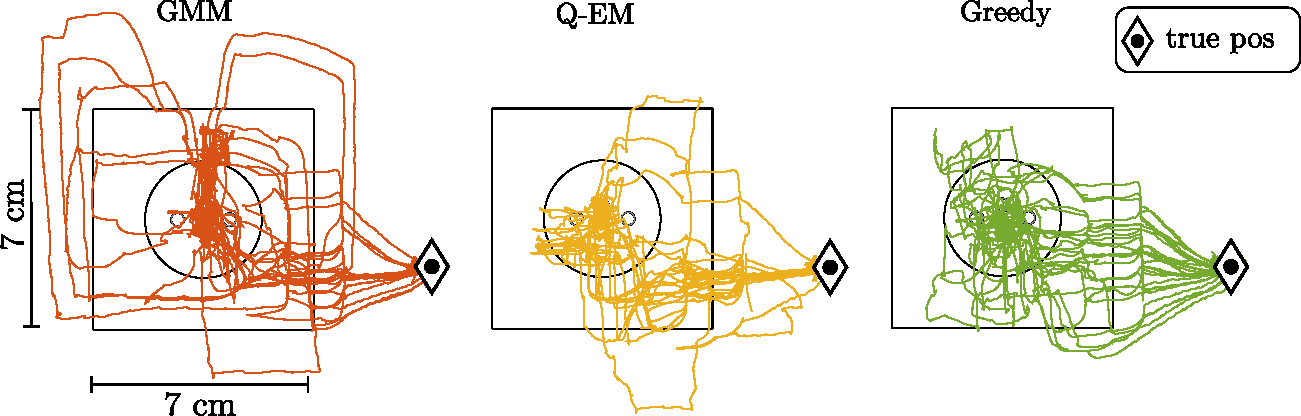
\includegraphics[width=\textwidth]{./ch4-PiH/Figures/Results2/socket_connection_A.pdf}}
    \caption{%(a) All three sockets have the same connector interface, but have different structures. Both 
   % socket A and B have an edge around the center whilst the surface of socket C is featureless and more elevated than the other two. 
    25 search trajectories for each of the three search policies for socket A. }
    \label{fig:real_policy}
\end{figure}


\begin{figure*}
 \centering
 \subfigure[]{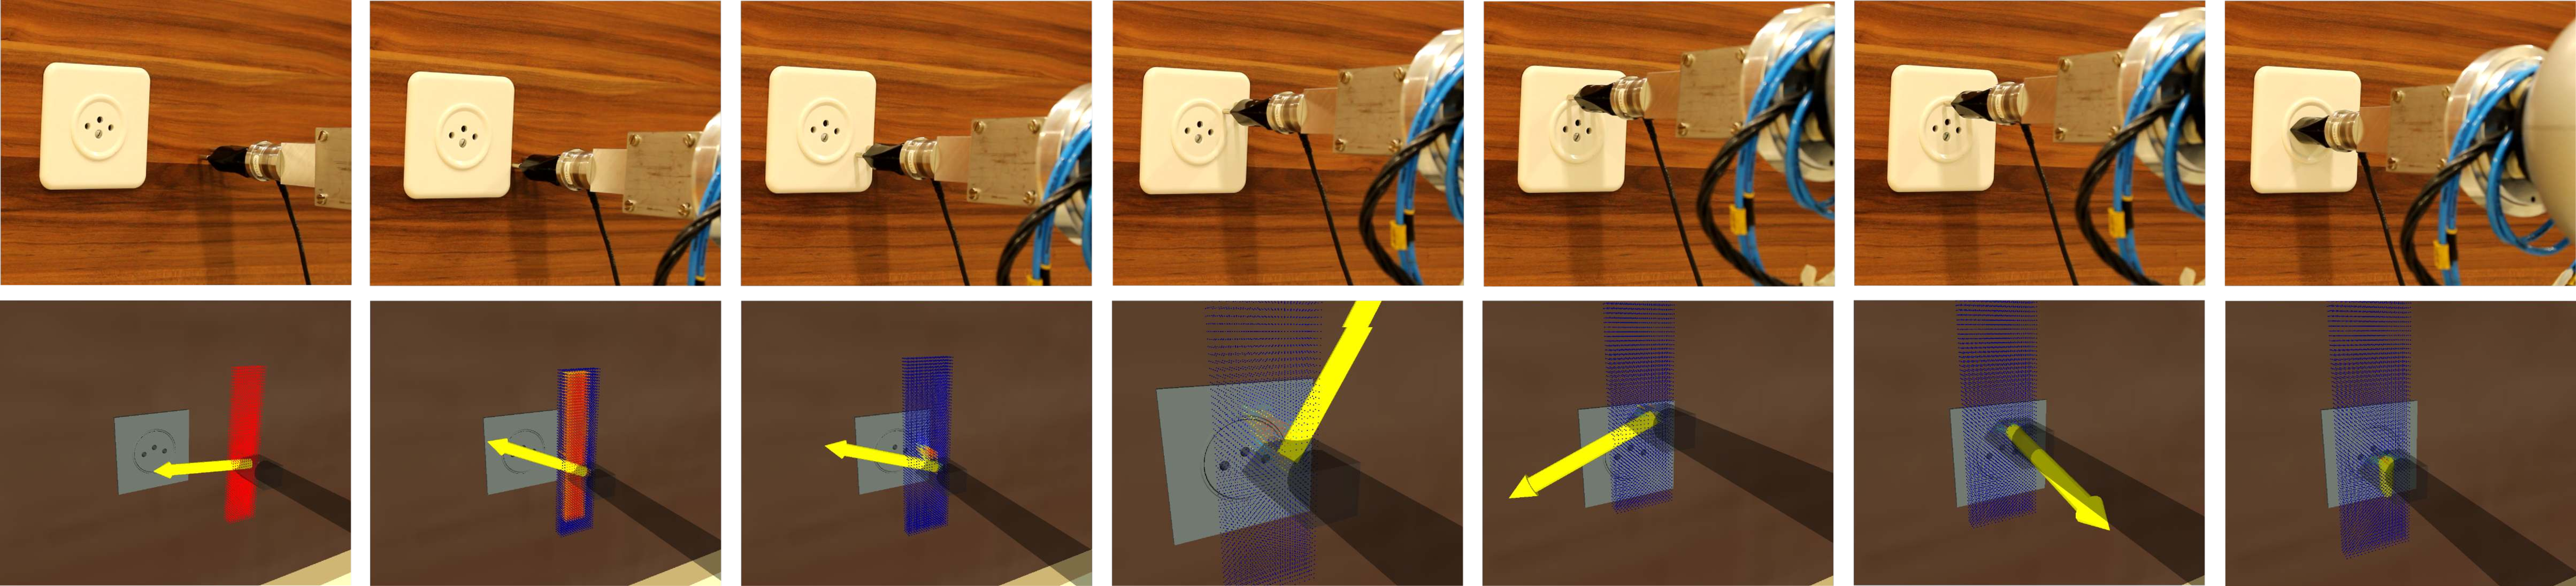
\includegraphics[width=0.95\textwidth]{./ch4-PiH/Figures/Results2/s1_sequence.pdf}}
 \subfigure[]{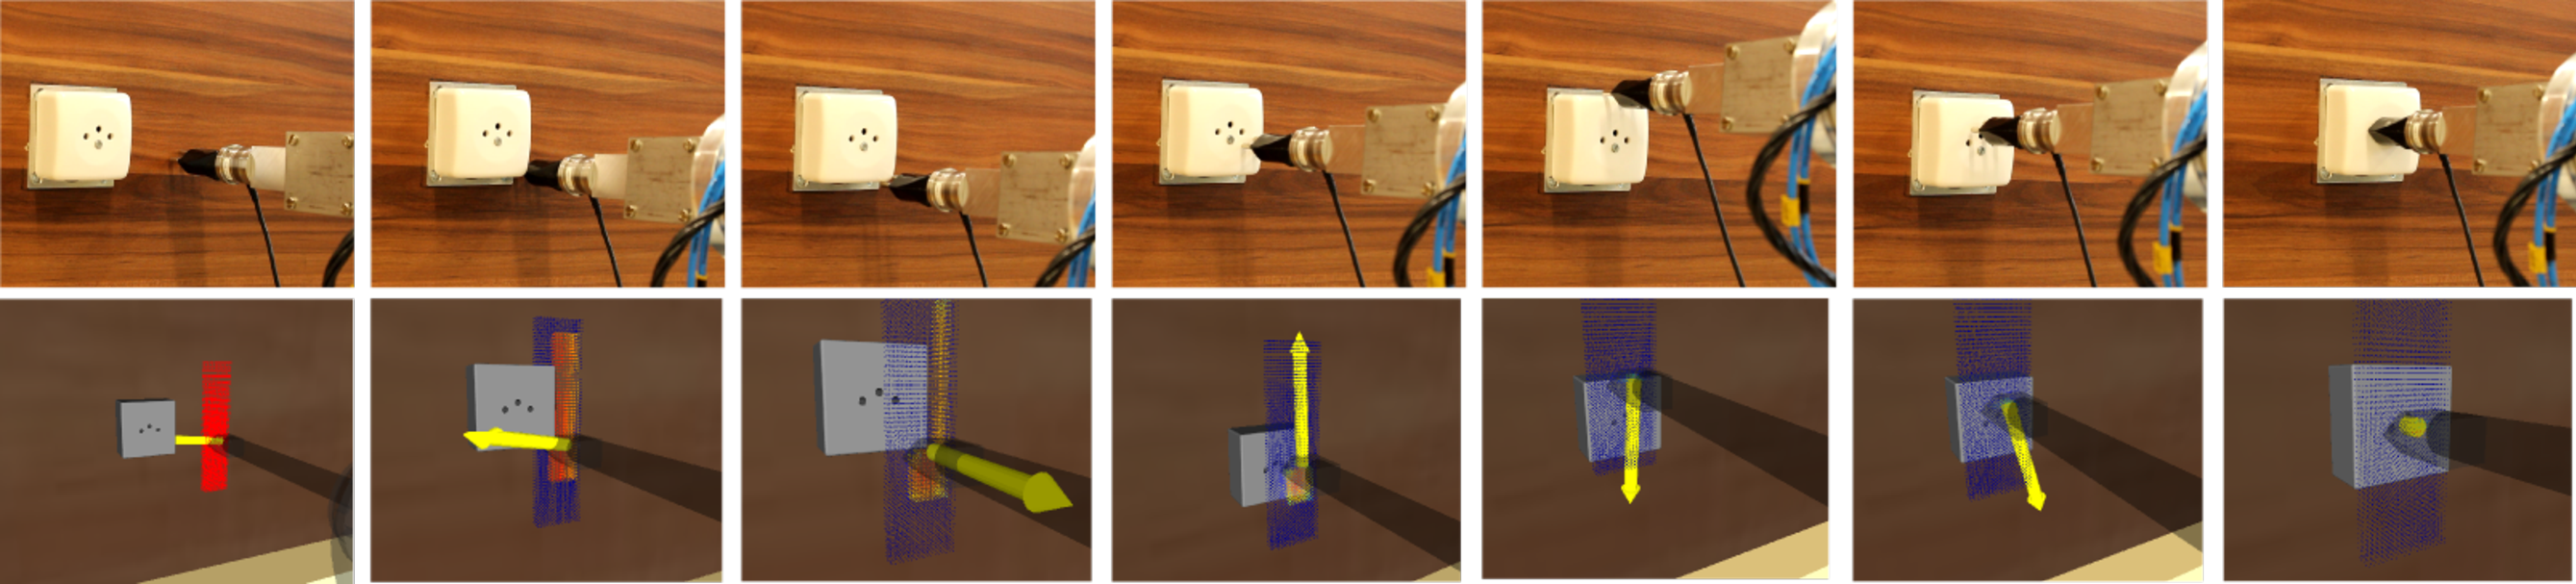
\includegraphics[width=0.95\textwidth]{./ch4-PiH/Figures/Results2/s2_sequence.pdf}}
 \caption{KUKA LWR4 equipped with a holder mounted with a ATI 6-axis force-torque sensor. (a) The robot's end-effector starts to the 
 left of socket A. The second row are screen captures of the ROS Rviz data visualiser in which we see the Point Mass Filter 
 (red particles) and a yellow arrow indicating the direction given by the policy. In this particular run, the peg remained in contact with the ring of the socket until 
 the top was reached before making a connection. (b) Same initial condition as in (a) but with socket C. The policy leads the peg down to 
 the bottom corner of the socket before going the center of the top edge, localising itself, and then makes a connection.}
 \label{fig:real_pictures}
\end{figure*}

\begin{figure*}
 \centering
   \subfigure[]{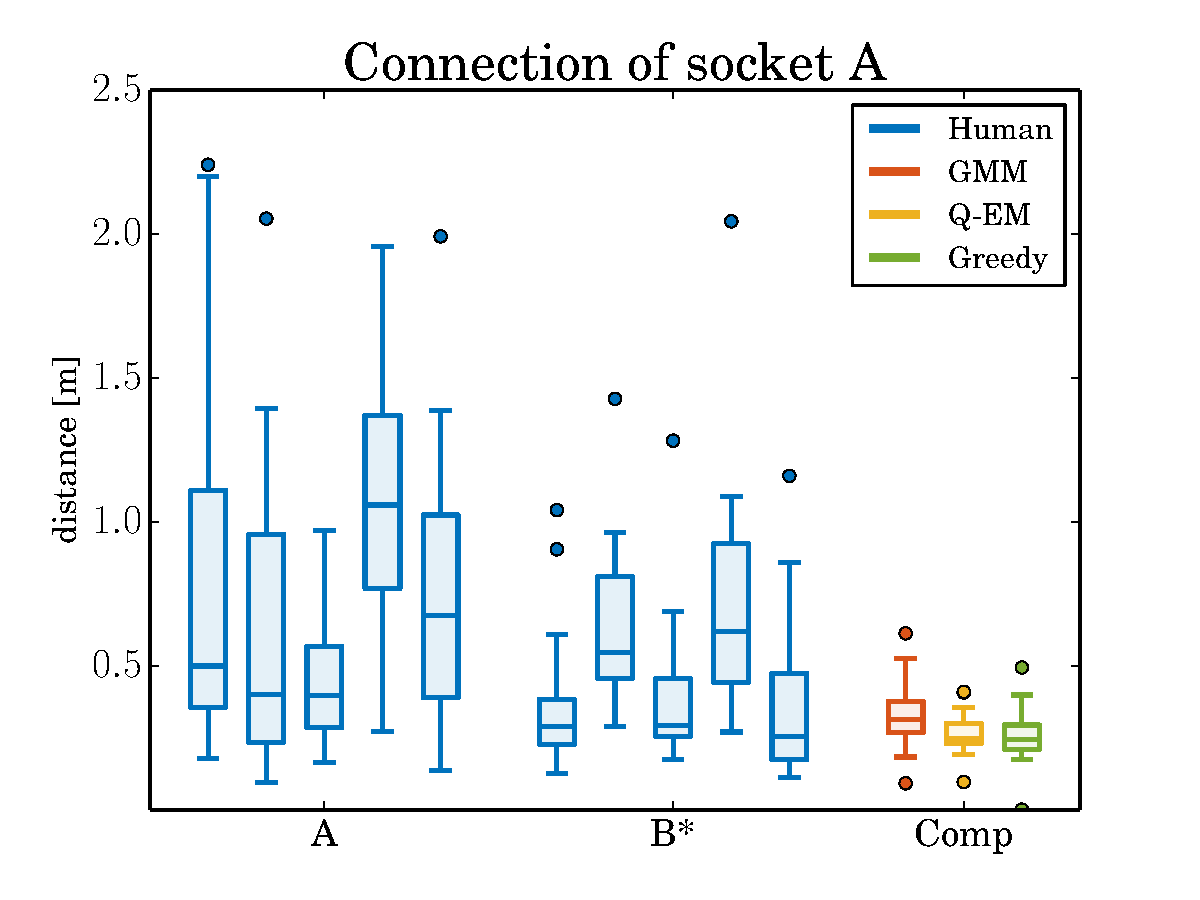
\includegraphics[width=0.3\textwidth]{./ch4-PiH/Figures/Results2/real_exp_socketA.pdf}}
   \subfigure[]{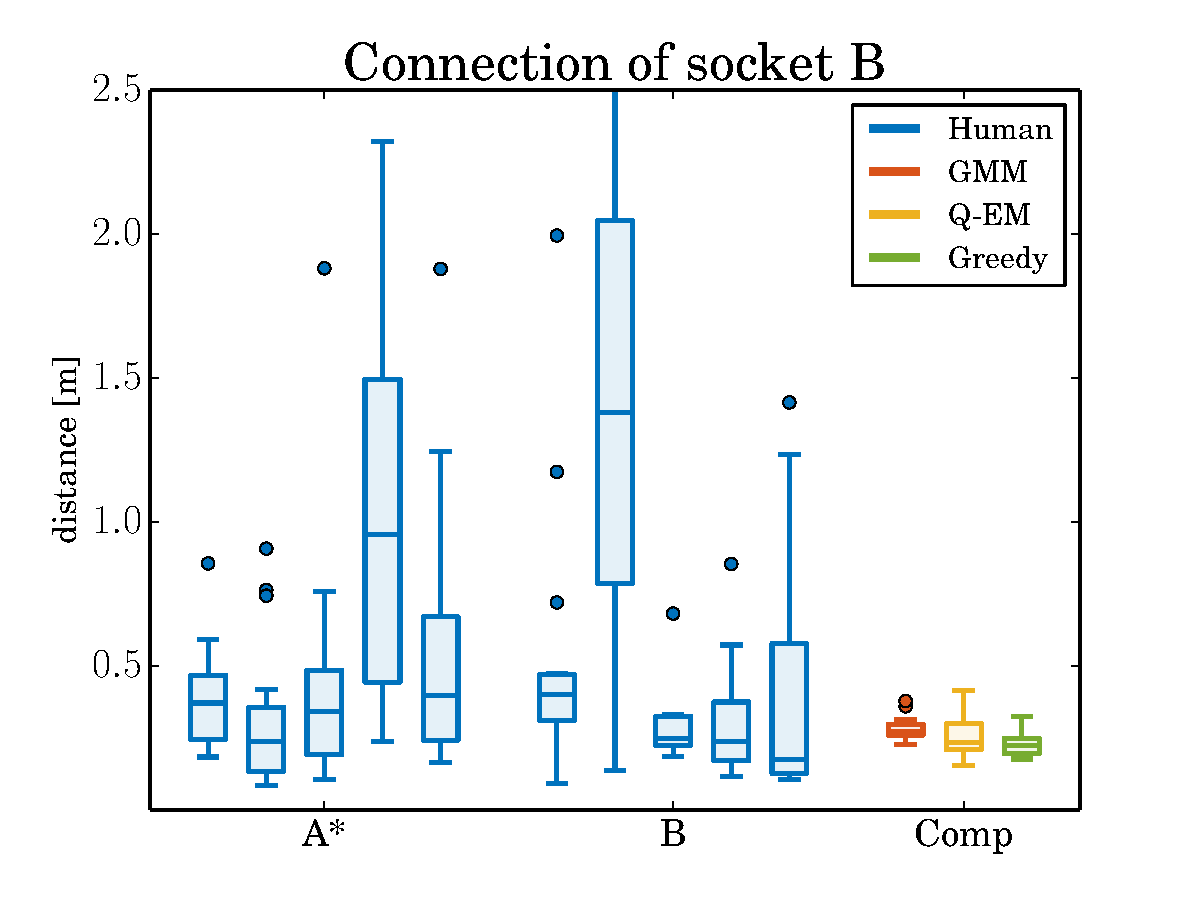
\includegraphics[width=0.3\textwidth]{./ch4-PiH/Figures/Results2/real_exp_socketB.pdf}}
   \subfigure[]{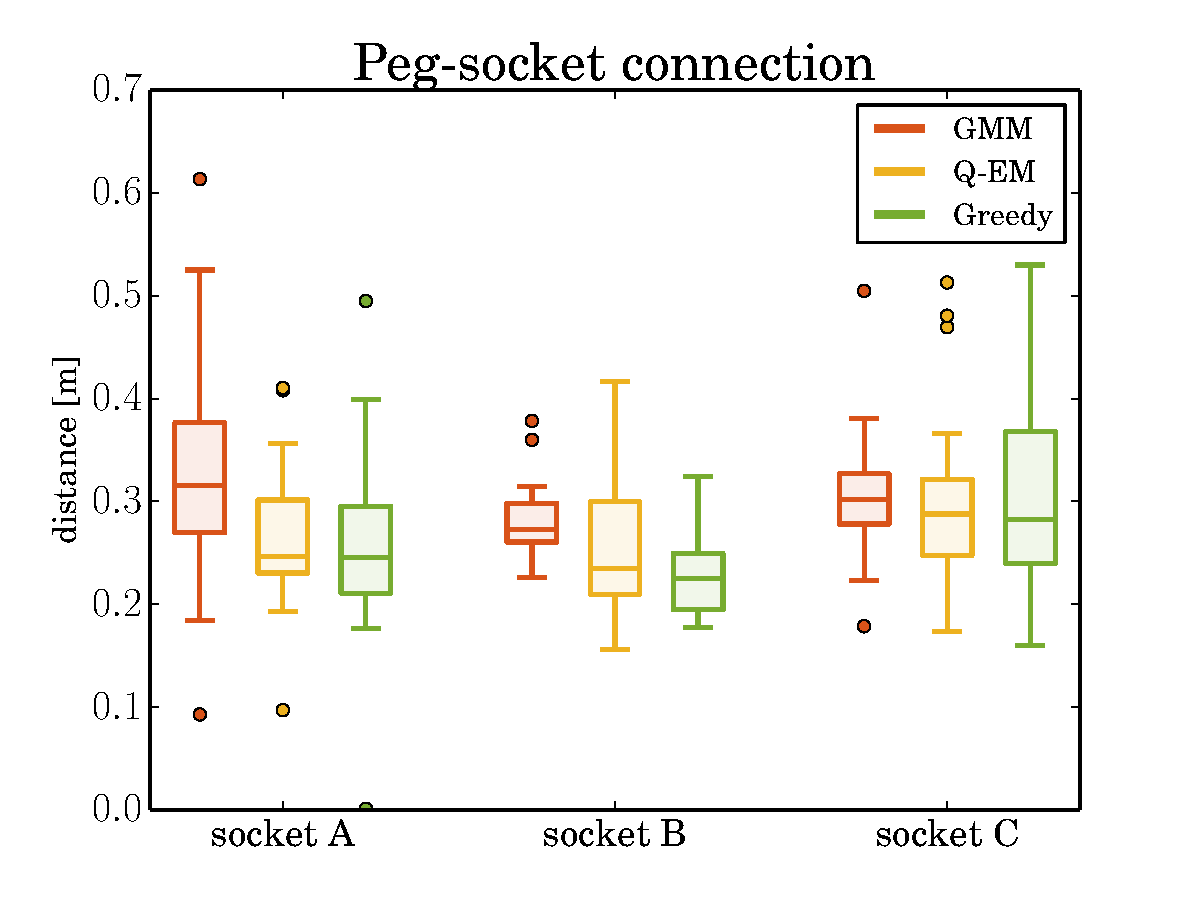
\includegraphics[width=0.3\textwidth]{./ch4-PiH/Figures/Results2/peg_socket_connection.pdf}}
  \caption{Distance taken to connect peg to socket once the socket is localised. (a) \textbf{Socket A}. The human 
  Group A are the set of teachers who first started with socket A, they did not have any other training before hand. Group 
  B\textsuperscript{*} first gave demonstrations on Socket B before giving demonstrations on Socket A. Group B\textsuperscript{*}
  is better than group A at doing the task. This is most likely a training effect. However all policy search methods are far better
  at connecting the peg to the socket. (b) \textbf{Socket B}. Both groups A\textsuperscript{*} and B are similar in terms 
  of the distance they took to insert the peg into the socket and as was the case for (a), the search policies travel less to accomplish 
  the task. (c) Distance taken (measured from point of contact of peg with socket edge) to connect the peg to the socket.  } 
  \label{fig:real_statistics}
\end{figure*}

The GMM and Q-EM policies are able to generalise to both socket B and C. The reason is that the geometric shape and connector interface of the 
two sockets are similar to socket A. The local force modulation of the policies vector field, which isn't learned, allows to get over edges and obstacles
whilst trying to maintain a constant contact force in the x-axis. This modulation makes it possible for the peg to get on top of socket C.
In Figure \ref{fig:real_statistics} (c) we illustrate the statistics of the distance taken to establish a connection for all three sockets. 
The point of interest is that both the GMM and Q-EM algorithms do better than the Greedy approach for socket C. Socket C has no informative 
features on its surface and as a result myopic policies will perform poorly as it is the case for the Greedy policy. However for socket A 
and B, the Greedy policy performs better. Both these two sockets have edges around their connector point allowing for easy localisation. 
It can also be seen that most search methods perform better on socket B than A, since the funnel shape connector helps in maintaining the peg 
within the vicinity of the socket's holes. 


The search discrepancy between the performance of the humans and search policies can be attributed to many causes. One plausible reason is that 
that the PMF probability density representation of the belief is too accurate with respect to what human teachers can represent. 
The noise motion noise parameter was fixed to be proportional to the velocity. The robot moves at gentle pace ($\sim1$ cm/s) as oppose to some of the human subjects. We
are fare less precise than the KUKA which has sub-millimetre accuracy.

\section{Discussion \& Conclusion}\label{ch4:conclusion}
% Recapulate what we did 
%
%	We learned a 
%
%

In this work we learned search policies from demonstrations provided by human teachers for a task
which consisted of first localising a power socket (either socket A, B or C) and then connecting it with a plug. Only haptic information 
was available as the subjects were blindfolded. We made the assumption that the position belief of the human teachers 
was initially uniformly distributed in a fixed rectangular region which they were 
informed off and is considered prior knoweldge. All subsequent beliefs were then updated in a Bayesian recursion 
using the measured velocity, obtained from a vision tracking system, and wrench acquired from a force torque sensor attached 
to the plug. The filtered probability density function, represented by a Point Mass Filter, was then compressed to the 
most likely state and entropy.

Two Gaussian Mixture Model policies where learned from the data recorded, during the teaching by the human subjects . 
The first policy, called Q-EM, was learned in an Actor-Critic RL framework in which a value function was learned over 
the belief space which was then used to weigh training datapoints in the M-step update of Expectation-Maximisation (EM). The second 
policy, called GMM, was learned using the standard EM algorithm, considering of all training data points equally,
following in the footsteps of our initial approach \cite{Chambrier2014}. Both the Q-EM and GMM policies we trained 
with data solely from demonstrations of the search with socket A.

We evaluated 4 different aspects of the learned policies. Firstly, we evaluated which of three policies, Q-EM, GMM and a Greedy policy, 
took the less distance to find the socket. We concluded that across three different Experiments the Q-EM algorithm was always 
the best. It was clear that the Q-EM policy was less random and more consistent that the GMM policy as it tried to enter in 
contact with the table at the same height as the socket, thus increasing the chances of finding it.

Secondly, we tested the importance of the data provided by the human teachers. We took the worst two subjects and trained an
individual GMM and Q-EM policy for each of them. We found that the performance of the Q-EM was better than the GMM in terms 
of distance travelled to find the socket. When qualitatively evaluating the the trajectories of the GMM with respect to the 
Q-EM for the worst subject, it is clear that the Q-EM policy managed to extract a search pattern, which was not the case 
for the GMM policy. We also tried to learn a Q-EM policy from the data provided by a Greedy policy with explorative noise 
and we found no improvement. From these results we conclude that the exploration and exploitation aspects of the trajectories 
provided by the human teachers is necessary.

Thirdly we tested whether the two policies were able to generalise to a different socket location. Under a specific condition
which we called \textit{Fixed} both policies were significantly better than the Greedy policy. However for the \textit{Center}
and \textit{Left} initial condition the Greedy policy was better. For the initial conditions in which the Greedy policy will 
enter in contact with the wall at an early stage will, it will do better than the GMM and Q-EM.  The reason being that 
the actions taken by the Greedy policy in this setting will always result in a decrease of entropy when the location
of the socket is close to a corner, as oppose to being in the center of the table.

Fourthly we evaluated the three policies on the KUKA LWR4 robot. First it the policies all did better than the human 
teachers. For socket A, which both the GMM and Q-EM policies were trained on, there is no clear distinction between 
the Q-EM and Greedy policy. On socket B, which was novel, the Greedy policy did better than the statistical controllers, 
which we hypothesis was a result of the funnel which would make it easier for a myopic policy. For socket C, both the 
GMM and Q-EM policies do better. The reason was that socket C, has no features on its surface, thus being a disadvantageous 
for a myopic policy.

We concluded by making the observation that by simply adding a binary reward function in combination with 
data provided by human demonstrations, with Fitted reinforcement learning, we can learn a better policy without 
the need of doing expensive exploration-exploitation  rollouts traditionally associated with reinforcement learning and 
designing complicated reward functions. This is especially advantageous when few demonstrations are available.

\section{Appendix}
\subsection{EM policy search}\label{app:lb}
Steps taken to make a policy $pi_{\Para}(\U,\B)$ maximise the objective function, $J(\Para)$.
The policy will be maximised with respect to the lower bound of the cost function $J(\Para)$:
\begin{align}
  J(\Para') &= \sum_{i \in \mathbb{T}} \pi_{\Para'}(\Ui,\Bi)\, R(\Ui,\Bi) \nonumber\\ 
	   &= \sum_{i \in \mathbb{T}}  \frac{\pi_{\Para'}(\Ui,\Bi)}{\pi_{\Para}(\Ui,\Bi)} \, \pi_{\Para}(\Ui,\Bi) \, R(\Ui,\Bi)
\end{align}

where $\mathbb{T}$ is the set of all rollouts. Next we take the logarithm and make use of Jensen's inequality and move the logarithm into the 
summation.

\begin{align}
  \log( J(\Para') )  &= \log \sum_{i \in \mathbb{T}} \frac{\pi_{\Para'}(\Ui,\Bi)}{\pi_{\Para}(\Ui,\Bi)} \, \pi_{\Para}(\Ui,\Bi) \, R(\Ui,\Bi) \nonumber \\
		     & \geq \sum_{i \in \mathbb{T}}\log\Bigg( \frac{\pi_{\Para'}(\Ui,\Bi)}{\pi_{\Para}(\Ui,\Bi)}\Bigg) \, \pi_{\Para}(\Ui,\Bi) \, R(\Ui,\Bi) \label{eq:lower_bound}
\end{align}

The new cost function be derived by taking derivative with of the lower bound of $\log(J(\Para))$ with respect to its parameters.
We take the derivative of the lower bound of $\log(J(\Para'))$, Equation \ref{eq:lower_bound}, with respect to $\Para'$ and set it to 
zero such to maximise the cost function.

\begin{align}
 &\nabla_{\Para'}  \log( J(\Para') ) = \nonumber\\
 &\sum_{i \in \mathbb{T}} \nabla_{\Para'} \log\big( \pi_{\Para'}(\Ui,\Bi)\big) \, \pi_{\Para}(\Ui,\Bi) \, R(\Ui,\Bi) \nonumber \\
				    & - \underbrace{ \nabla_{\Para'} \log\big( \pi_{\Para}(\Ui,\Bi)\big) \, \pi_{\Para}(\Ui,\Bi) \, R(\Ui,\Bi)}_{\color{red} =0} \nonumber \\
				    &= \sum_{i \in \mathbb{T}} \nabla_{\Para'} \log\big( \pi_{\Para'}(\Ui,\Bi)\big) \, \pi_{\Para}(\Ui,\Bi) \, R(\Ui,\Bi) \nonumber \\
				    &= \mathbb{E}_{\pi_{\Para}(\U,\B)} \Big\{ \nabla_{\Para'} \log\big( \pi_{\Para'}(\Ui,\Bi)\big)\, R(\Ui,\Bi) \Big\}
\end{align}

\begin{align}
 \nabla_{\Para'}  \log( J(\Para') ) &= \mathbb{E}_{\pi_{\Para}(\U,\B)}\Big\{R(\Bi,\Ui)  \sum_{t=0}^{T}\nabla_{\Para'}\log \pi_{\Para'}(\Ui,\Bi)\Big\}\\
				    &= \sum\limits_{i=1}^{N} \sum\limits_{t=0}^{T^{[i]}} \nabla_{\Para'}\log \pi_{\Para'}(\U^{[i]}_t,\B^{[i]}_t) \, Q^{\pi}(\U^{[i]}_t,\B^{[i]}_t) \label{eq:grad_log_cost_2}
\end{align}

The reader is referred to \cite{rl_gradient_survey_2013} for more details regarding Expectation-Maximisation and policy search in reinforcement learning.

\subsection{Q-EM for GMM derivation}\label{app:grad}

Making the substitution $\X = (\U,\B)^{\mathrm{T}}$ (small abuse of notation) and  insuring a positive Q-function, $Q^{\pi}(\X^{[m]}) \geq 0$
and by setting the derivative of Equation \ref{eq:grad_log_cost_2} to zero and solving for the parameters
$\Para=\{w,\boldsymbol{\mu},\boldsymbol{\Sigma}\}$ we get a new weighted Maximisation updates in EM:

\begin{align}
\nabla_{\MuK} \log J(\Para) =& \sum\limits_{m=1}^{M} \alpha(z_{mk})\, Q(\Xm)\, \invSigK (\Xm - \MuK) = 0 \nonumber \\
			 \MuK_{\textrm{\textbf{new}}} =& \frac{\sum\limits_{m=1}^{M} \alpha(z_{mk})\, Q(\Xm)\, \Xm }{\sum\limits_{j=1}^{M} \alpha(z_{jk})\, Q(\X^{[j]})}
\end{align}

where $\alpha(z_{mk})$ is the responsibility factor, denoting the probability that data point $m$ is a member of the 
Gaussian function $k$.

\begin{equation}
 \alpha(z_{mk}) = \frac{w^{[k]} \cdot g(\Xm;\MuK,\SigK)}{\sum\limits_{j=1}^{K}w^{[j]} \cdot g(\Xm;\boldsymbol{\mu}^{[j]},\boldsymbol{\Sigma}^{[j]})}
\end{equation}

\begin{equation}
   \SigK_{\textrm{\textbf{new}}} = \frac{\sum\limits_{m=1}^{M} Q(\Xm) \alpha(z_{mk}) (\Xm - \MuK)(\Xm - \MuK)^{\mathrm{T}} }{ \sum\limits_{j=1}^{M} Q(\X^{[j]})\, \alpha(z_{jk}) }
\end{equation}

\begin{equation}
  w^{[k]}_{\textrm{\textbf{new}}} = \frac{\sum\limits_{m=1}^{M} Q(\X^{[m]})\, \alpha(mk)}{\sum\limits_{j=1}^{M} Q(\X^{[j]})}
\end{equation}

%\subsection{M-step}\label{app:Q-EM}
%Given a set of points $\X = (\U,\B)^{\mathrm{T}}$ and  a positive Q-function, $Q^{\pi}(\X^{[m]}) \geq 0$
%and by setting the derivative of Equation \ref{eq:grad_log_cost} to zero and solving for the parameters
%$\Para=\{w,\boldsymbol{\mu},\boldsymbol{\Sigma}\}$ we get a new weighted Maximisation updates in EM:
%\begin{align}
% w^{[k]}_{\textrm{\textbf{new}}} &= \frac{\sum\limits_{m=1}^{M} Q^{\pi}(\X^{[m]})\, \alpha(z_{mk})}{\sum\limits_{j=1}^{M} Q^{\pi}(\X^{[j]})} \\
% \MuK_{\textrm{\textbf{new}}}     &= \frac{\sum\limits_{m=1}^{M} \alpha(z_{mk})\, Q^{\pi}(\Xm)\, \Xm }{\sum\limits_{j=1}^{M} \alpha(z_{jk})\, Q^{\pi}(\X^{[j]})} \\
% \SigK_{\textrm{\textbf{new}}}    &= \frac{\sum\limits_{m=1}^{M} Q^{\pi}(\Xm)\, \alpha(z_{mk})\, (\Xm - \MuK)(\Xm - \MuK)^{\mathrm{T}} }{ \sum\limits_{j=1}^{M} Q^{\pi}(\X^{[j]})\, \alpha(z_{jk}) }
%\end{align}
%$\alpha(z_{mk})$ is the responsibility factor, denoting the probability that data point $m$ is a member of the 
%Gaussian function $k$ (see \cite[Chap. 9]{Bishop_2006}).

\subsection{Unbiased estimator}\label{app:unbiased_delta}

%\begin{equation}
%  \delta^{\pi}_t = r_{t+1} + \gamma V^{\pi}(b_{t+1}) - V^{\pi}(b_t) \\
%\end{equation}
The temporal difference error is an unbiased estimate of the advantage function:
\begin{align}
  \displaystyle \mathop \mathbb{E}_{\pi_{\Para}} \{ \delta^{\pi}_t|b_t,u_t\} &=  \mathop\mathbb{E}_{\pi_{\Para}}\{ r_{t+1} + \gamma V^{\pi}(b_{t+1})|b_t,u_t\} - V^{\pi}(b_t) \nonumber \\
									   &= Q^{\pi}(b_t,u_t) - V^{\pi}(b_t) \nonumber \\
									   &= A^{\pi}(b_t,u_t)
\end{align}
